\documentclass{article}
\usepackage[left=2cm, right=2cm, top=1cm]{geometry}
\usepackage[utf8]{inputenc}
\usepackage{amsmath}
\usepackage{enumitem}
\usepackage{float}

\title{Hyperspectral Imaging Biodiversity}
\author{Hannah Gallagher}
\date{October 13th, 2024}

\usepackage{natbib}
\usepackage{graphicx}

\begin{document}

\maketitle

\section{Introduction}

%Convolution 
%Eigenvalues Eigenvectors 
%Discrete fourier transform 
%Continuous transform 
%Vector basis 
%Circulant matrix
%Euler relation



% Hot keys to remember: command / on a mac comments highlighted code in and out.
%Nugget the snowman wishes you good luck on your research!

%\begin{figure}[h!]
%\centering
%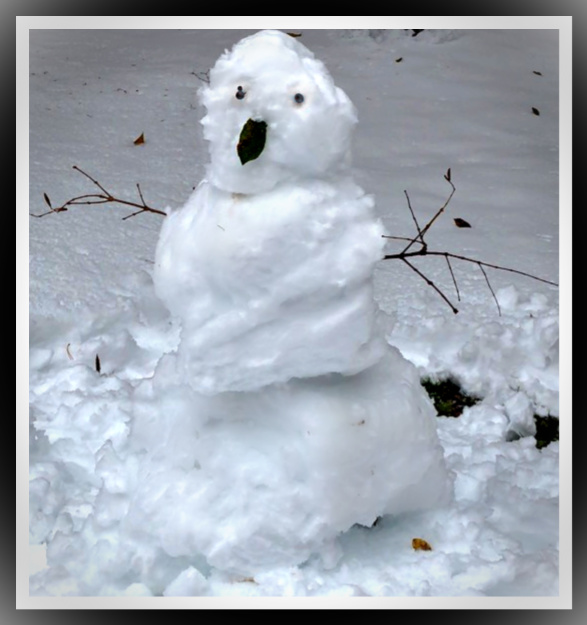
\includegraphics[scale=1]{Nugget.jpg}
%\caption{Nugget the Snowman}
%\label{fig:Nugget}
%\end{figure}

\section{Given Information, Key Terms, and Things to Remember} 
\begin{itemize}
\item Hyperspectral Imaging
\item ENVI
\item Radiance
\item https://scienceandtechnology.jpl.nasa.gov/dr-marc-simard
\item Parameterization of stuff and that NASA problem 7 on pset 2
\item Solid Angle 
\item All the different definitions around radiance, irradiance, radiant intensity etc.
\item 4PIX
\item Edge Detection
\item Global Warming
\item Salt Marshes protect ecosystems
\item LiDAR shows more fine details


% \begin{figure}[h!]
% \centering
% 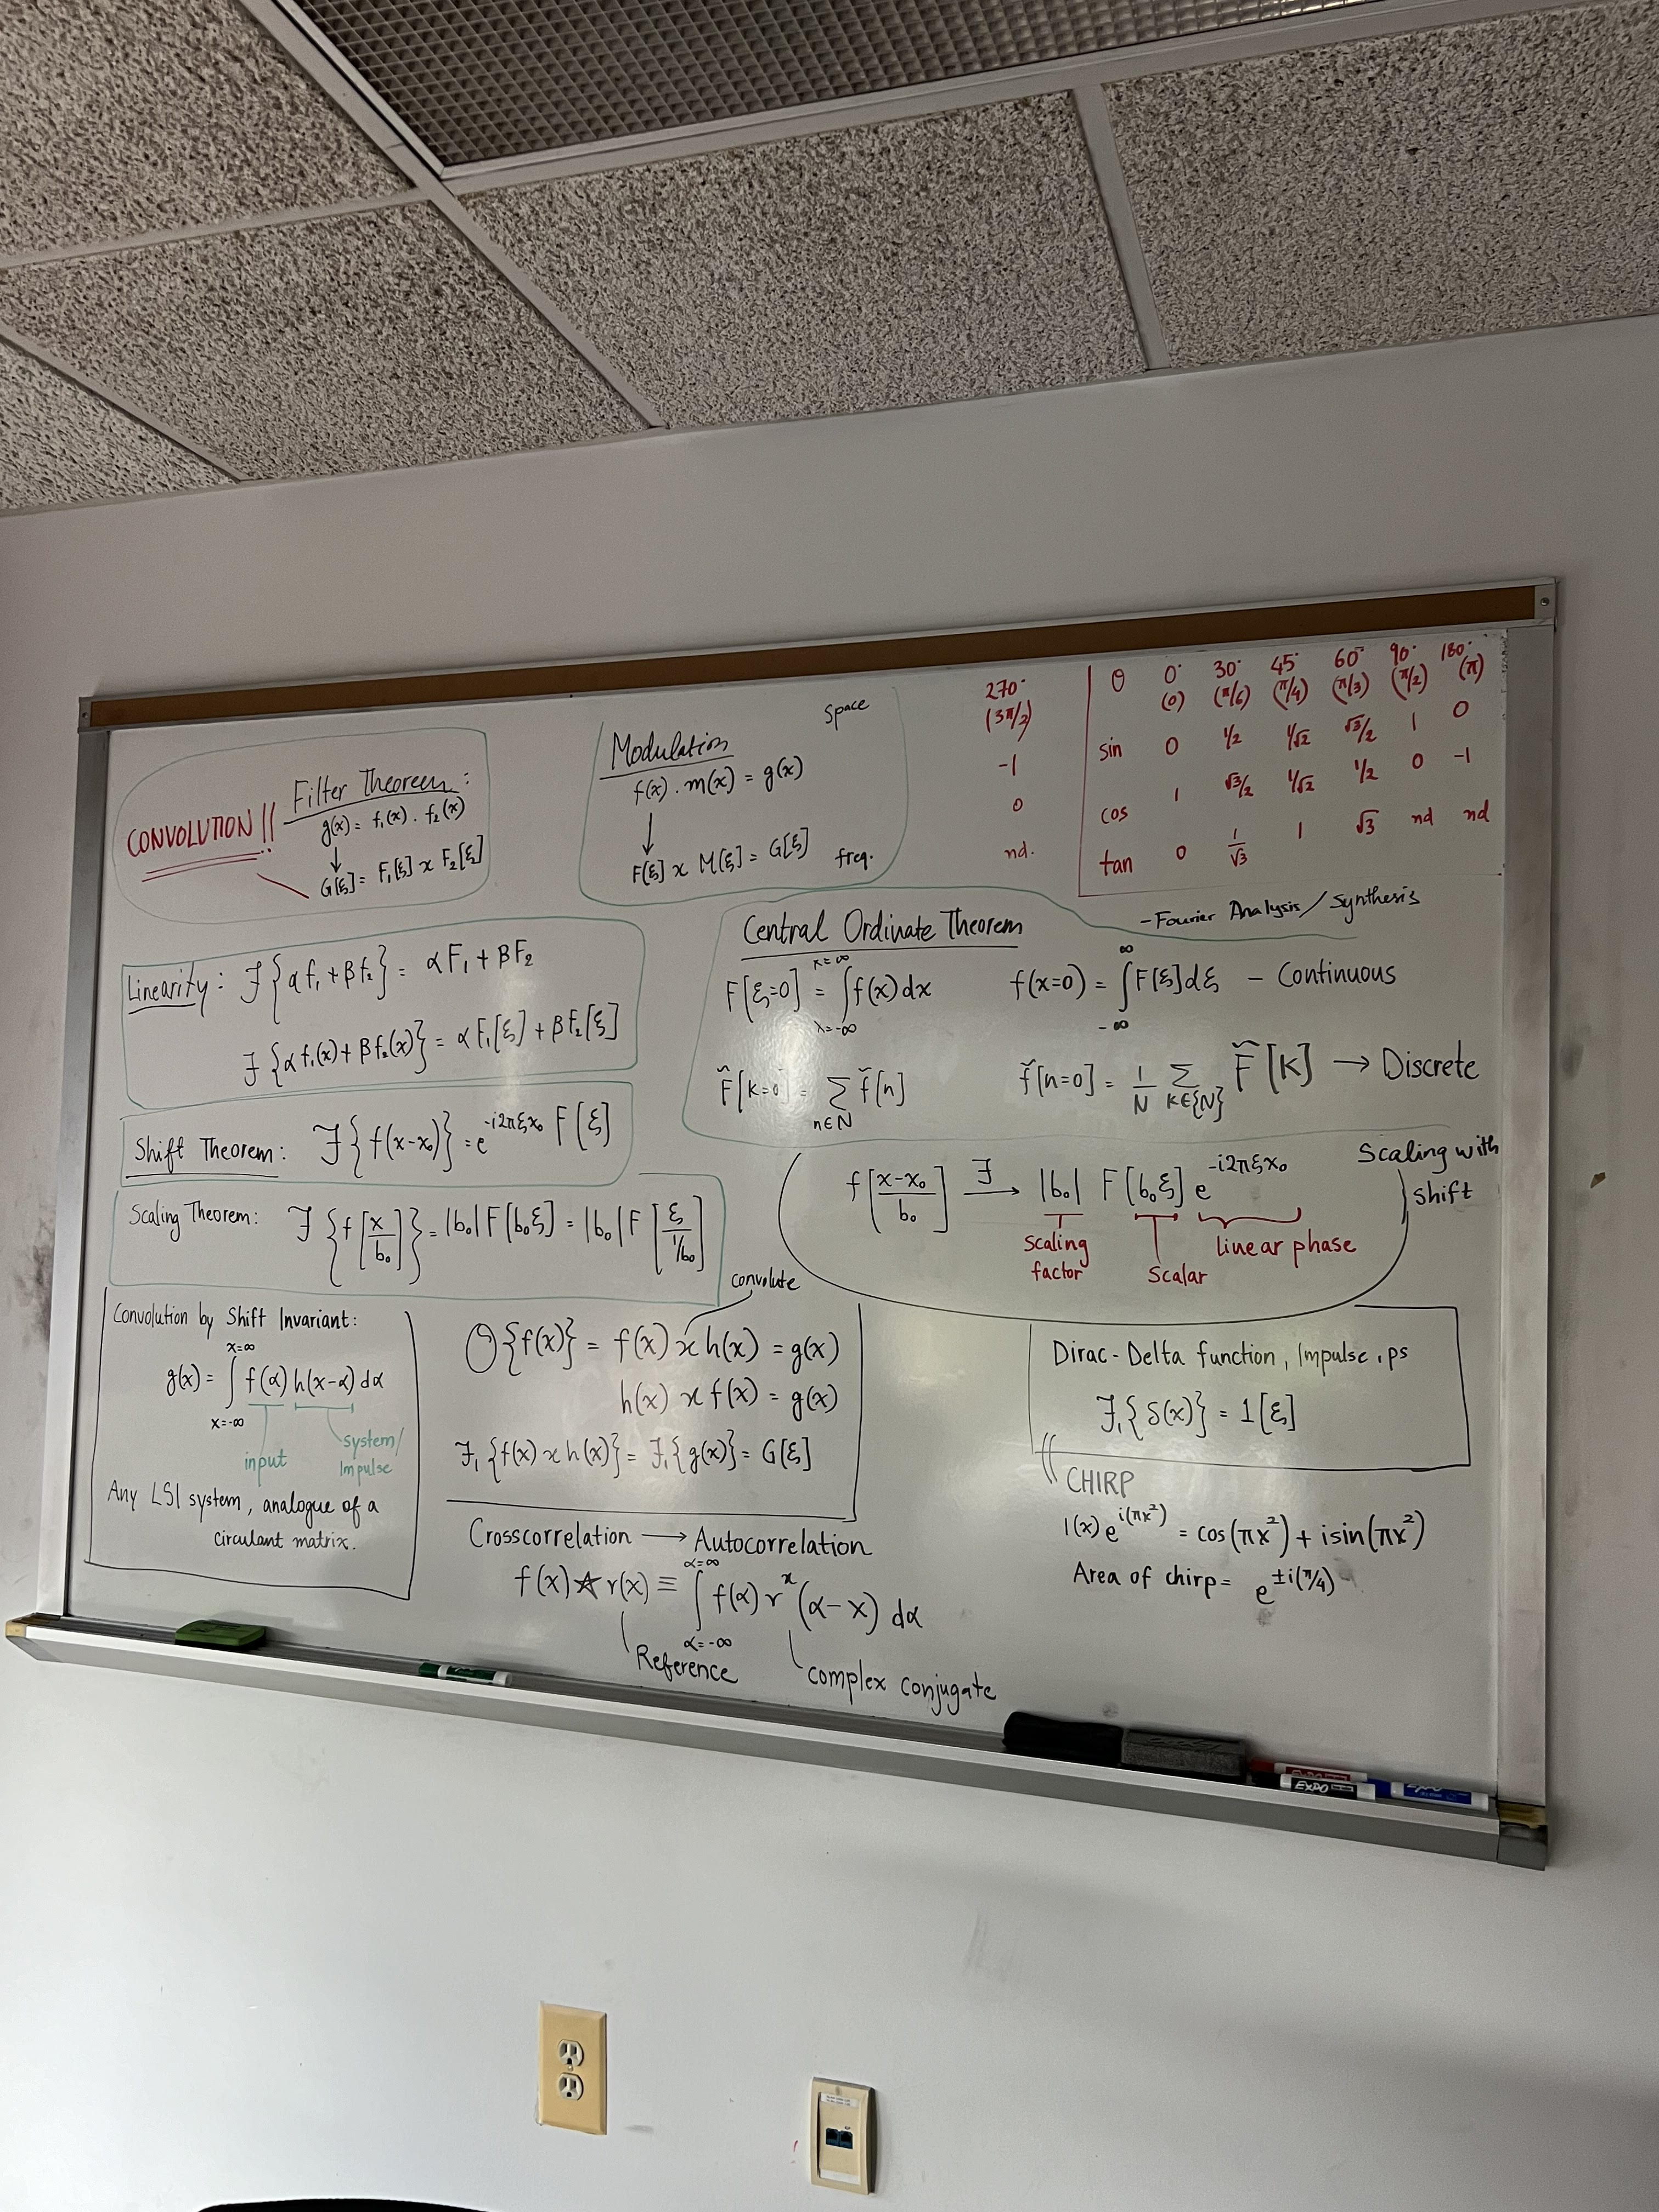
\includegraphics[scale=.20]{Fourier/unnamed.jpg}
% \caption{Easton Syllabus}
% \label{fig:Snowman4}
% \end{figure}


 
\end{itemize}

\clearpage

\section{Day by Day}

\subsection{October, 2024}
(Beginning stages in another document along with weekly GRIT meetings are in a google doc.)
Nayma wrapping up research and explaining how to use the dat files and open shape files in ENVI as they all need to be present to view the file. 

\subsection{November 8th, 2024}
Finally achieved the mosaic image in ENVI during the research meeting. Asked about a hard drive to borrow.



\subsection{November 13th, 2024}
Research meeting after the second Fourier exam. Received the hard drive to borrow as it was okayed to be cleared.

\subsection{November 15th, 2024}
Week frees up a little bit and made plans to read more papers on hyperspectral imaging, red edge, and ENVI over the weekend. Quick check in with Dr. Bachmann to ask about possible meeting times. Grant due Monday for Dr. Bachmann so Tuesday meeting planned. (Will also have to be quick).

\subsection{November 21st, 2024}
Undergraduate research presentation for AWM and PiRIT. Practiced public speaking and speaking about research. 

\subsection{November 22nd, 2024}
Bowling with Pure Physicists.    

\subsection{November 23rd, 2024}
Went to High Acres Nature Area. (HANA) 

Studied how I could learn about tree health in marshes from the ground level as everything I'm working in is too small. Need a broader idea to get started. 

See end of document to see pictures from the tree study. 


\subsection{November 26th, 2024}
Studied and read the Radiometry textbook 2-5 again. 

\subsection{November 27th, 2024}
Had the idea to use the human vision review model to do this lit review. Read a few papers that were review papers, but they really only spoke on different software. Looked over the lab data and that may help in the future knowing those fundamentals. 



\subsection{November 28th, 2024}
Read more papers about software, such as random forest, not very insightful as I have already used random forest in past research. Anything done with machine learning was glossed over.  

\subsection{November 29th, 2024}

(Early Morning) Application of leaf multispectral analyzer in comparison to hyperspectral device to assess the diversity of spectral reflectance indices in wheat genotypes: Sunlight is important in analyzes the health of an ecosystem as it is needed for photosynthesis. 
Plant Senescence Reflectance Index. 

(Noon) Read Radiometry Textbook Chapters 7-10 again on the drive home from Thanksgiving. Various relevance to Radiometry as Photometry is not the focus. 

Crop yields paper and fertilizer levels differences\\
(Evening) 10 year high school reunion. Spoke about research and had a few ideas for research topics more relating to human vision. 
Went to bed early and was too tired to look at anything. 


\subsection{November 30th, 2024}
Spoke about research with neighbors at annual Christmas Tree party. Practice for explaining topics and thoughts. Importance of detection of dry leaves for fires as wind blew the leaves towards the fire. Browsed papers when home about research papers relating to campfire smoke in eyes and detectability in satellite, hyperspectral imaging etc. Thought more about Volcanic atmospheric conditions. 


\subsection{December 1st, 2024}
Spent the early morning watching Radiometry lectures again from the midterm to Thanksgiving. Took notes in LaTeX on what was mentioned and emphasized in each lecture. Looked through the homework again. Found the relevant lecture that mentioned all of the important practice problems for the homework.

Continued to work on the lab. Found relevant lectures pertaining to that. 

Continued  to keep up with Dr. Bachmann Google Scholar notifications. Read those papers and then extrapolated from the related OSA papers in one of the beach studies from 2015. Found a study on the development of white radishes in China which require ample nitrogen which relates to Nayma's work. 

Browsed ENVI's abilities and help menu. Downloaded more photos. 

My dad wanted a marble ball bee water feeder for Christmas and I looked up some papers on how it worked. Apparently bees see in UV light. I already know a lot about bees so that could be an avenue. 

\subsection{December 2nd, 2024}

Early Morning: Read papers on hyperspectral and LiDAR imaging of bee and floral biodiviersity.

QUESTION: 
How can Lauren detect the snails she's studying for their biodiviersity in the marshes? Aren't they too small? They're most likely brown so in a muddy environment they probably blend in. Could she simply be looking for the plants or looking at different pictures that are closer to the ground?

Plan: 
Continue to work on Radiometry Lab and Homework. Do easy questions for Fourier. Submit final draft outline for Human Vision. Listen to more papers while grading etc. 

Tomorrow: Finish up Fourier homework. Work on Lab and ask questions. 

Wednesday: Go to seminar to ask questions and work on Radiometry Lab. 



\subsection{December 4th, 2024}
Group meeting and ask everything I had directly that was in this document. 

\subsection{December 5th, 2024}
Human Vision Final. 


Meeting with Dr. Bachmann. 
\subsection{December 6th,2024}
Radiometry lab cram as there was no other time to do the brunt of the work. Sleep deprivation and stress. 

\subsection{December 7th, 2024}
Recover from the lab. Three hours of sleep and then polish the lab to have better workmanship habits. 

Call it quits in the morning and nap. 

Caaught up on errands and everything pushed because of how busy the week was. Printed out review packet. Decorate tree to de-stress. 
Looked over lectures. Try to stay up, but was still sleep deprived and passed out watching a lecture. 

\subsection{December 8th, 2024}
Tried to memorize practical resolving power equations and grating equation. Paid attention to what was emphasized and not in lectures. 
Watched Radiometry lectures September 10th-November 7th 2024. Made folders and took screenshots of important moments and put them in each lecture day's folder. Worked a little to be able to afford retaking classes if necessary (kept me off my phone). 
Read textbook. Scalded left hand with coffee and went home. 
Wrote out solutions to hw number 1. Was worn out from the pain of the coffee burn so had to listen to old music to feel something and get re-motivated. Realized that I needed to listen to music earlier in the semester because it helped a lot. My original logic was that I would remember what was said in lectures if that was the only thing I listened to, but it probably made life too monotonous despite the lectures actually being fun with the random interjections.  

\subsection{December 9th, 2024}
Went through all the lectures for Radiometry. 
Studied with Muskan, Jason, Triya, and Aisha for Radiometry. 


\subsection{December 10th, 2024}
Studied for Fourier and Radiometry with Tony. We went over optical depth problems. Asked Dr. Easton questions for an hour about Fourier. 

\subsection{December 11th, 2024}
Studying for Radiometry. Wrote out all the homework problems and made a review sheet for everyone. 

\subsection{December 12th, 2024}
Radiometry Final Exam. Forgot about shot noise camera problem even though it was on my study sheet. Met with Dr. Easton later to ask questions for an hour. 

\subsection{December 13th, 2024}
Fourier Final Exam. I don't know what I got, but I remembered all the formulas and had thoughtful answers. I answered practically every problem. Bothered Dr. Easton for last minute questions before the exam. 

\subsection{December 14th, 2024}
Wrote a really good Human Vision review paper in less than a day on Migraines with aura. 


\subsection{December 15th, 2024}

Continued to read the paper that I found where Dr. Bachmann was cited. "The Reflectance of Solar Light from Natural Surfaces." 
Graded papers for Numerical Analysis as I put that off to get through finals which was approved by Dr. Lousto. 

I want to have at least 350 days where I committed to Github (they can be minor changes such as an update) so that no matter what the outcome of the semester is that I still have a plan and am being productive. I know I needed a break last year, but I did not work enough. 

\subsection{December 16th, 2024}
Got up early and finished grading the papers for Numerical Analysis. Caught up on Soleo work and started looking at my winter project...wishing for more hours. Returned to the gym and everyone said, "Hello stranger." 
I had classic talks with people about how I should help find water on Mars or asteroids. 

\subsection{December 17th, 2024}
Reviewed Radiometry slides and lectures (seventh time) for my own benefit. 
Meeting with Jan and Dr. Bachmann. 
Jan meeting went well and I can be a hybrid student. 

\subsection{December 18th, 2024}
Review anything that I missed in Radiometry in the early morning. Start winter project for Soleo. Back to doing more technical analytics now that I have bandwidth. 

Read five papers from the google drive for the research group. Including BRDF and soil moisture content. Hapke model papers seemed empty so I need to find a few on that on my own. 

\subsection{December 19th, 2024}
Focused on Soleo work. Did some QA on Allstate. Started my winter project and produced a spreadsheet for a point to start at for gaining new affiliates. Then I sent this finished spreadsheet to my boss and looked at SEMRush to do some analytics. 

Got Radiometry grade and processed it. Looked through some of the lectures to see where I went wrong. I did better in Fourier and that is objectively harder. Memorizing is clearly not my strong suit. Maybe I spent too much time on blackbody theories. Usually putting too much weight on a class usually has the opposite effect I want as then I am stressed. I'm not sure how it went this wrong though. Maybe the snow threw me off, but that shouldn't be a factor. I made the study document. I studied with people. I made flashcards. I watched the lectures a ton. I redid the homeworks. I highlighted the textbook throughout Thanksgiving break. Most of what was on the exam had something related to it in my study guide. I didn't know much about the coral problem, but I understood the theories. I reviewed the fundamentals in the second and third problem a ton. I probably should have gone in person since reading the problems took too long. 

It was all doable and possible. I am rusty with these fundamentals and being an A student, but undoubtedly I made progress this semester whether my grades reflect that or not. 

Downloaded chapter 2-8 of the Hapke Radiative Transfer textbook to decide if I can handle the material. 

\subsection{December 20th, 2024}
Clicked around to find SEMRush Traffic and referrals csv exports for Soleo. I have been catching up on doing the December calls for Allstate. 

The Elm story of the diseased trees in the 60's from my dad. Need to follow up to see some of these trees in HANA. 

I read through more of the radiative transfer book. I need to decide what other class to take, but they are all good options. It would help to read each book. 

%I had some car trouble today so hopefully it will not be a problem in the future. Good thing I am technically online student so I should be able to make it work if the jeep bites the dust. 

\subsection{December 21st, 2024}
%Ran errands, painted, wrote, attempted to ship present. Visited Grandma. 

Caught up on December's calls for Allstate. 

In BRDF Science Direct Papers Yamaguchi et al. I learned that snow avalanches are caused by "rain falling on snow" which would make the area heavier thus providing a stimulus to an avalanche. 

Emailed Grover for more information about the Optics course. I will have to wait until after the holiday to ask Dr. Messinger. 

%Need to cancel subscriptions. 

Watched youtube lectures on metrology to prepare for interview. 


\subsection{December 22nd, 2024}
Worked a little. Went bird watching in Hamlin and Braddock Bay area. Saw some snow geese...then hundreds of Canada geese. We spent sometime distinguishing between snow buntings and lapland longspurs. 

%Cleaned for the holidays and wrapped presents. 
%Small Holiday party at our place with Justin's friends. 

\subsection{December 23rd, 2024}
Worked on SEMRush. 
Found out that a textbook I've had for four years, that I got out of pure interest and knowing it was a prominent one, is a required textbook for Optics. 

\subsection{December 24th, 2024}
The holiday. %Read for fun. 

\subsection{December 25th, 2024}
The holiday. %Painted. 

\subsection{December 26th, 2024}
Looked at SEMRush. Read more of the optics textbook. 

\subsection{December 27th, 2024}
Read about hyperspectral research of blueberries in a drought. Continued to read the Fourier Optics Textbook (Chapter 3). Reviewed chapters 1-5ish of Radiative Transfer Textbook. 

\subsection{December 28th, 2024}
Read the rest of Chapter 3 and started Chapter 4 of the Goodman textbook. I need to do more reading on LiDAR point clouds...there has been too much focus on hyperspectral and I think I've been neglecting the LiDAR aspect of the project. 


\subsection{December 29th, 2024}
Fraunhofer diffraction in Goodman book. Read through chapter 5-6 of Radiative Transfer Textbook. 

\subsection{December 30th, 2024}
%QA Allstate Calls
Read Radiative Transfer book Chapters 6-7. Look through the Radiometry supplementary textbook before it expires on the 5th. 
%Finished the spreadsheet for SEMRush sites.
%Caught up on sleep. 
\subsection{December 31st, 2024}
Planned out 2025. Rang in the new year! 


\subsection{January 1st, 2025}
Pages read- 40
Radiative Transfer Chapter 6 
Goodman Optics Chapter 3-4 again. 

\subsection{January 2nd, 2025}
Read about coated particles for chapter 6.4 Radiative Transfer.

Chapter 4 Radiative Transfer. 
Chapter 7-8 Radiative Transfer. Reflectivity and Diffusivity. Lambert's Law. I need to review Legendre polynomials. 

\subsubsection{Google Drive Readings}
BRDF and Radiative Transfer Drive ScienceDirect
Read NEO - Evidence for aqueous altered surface - Keywords albedo. Low albedo asteroids. 
Pages read - 85 including Radiative Transfer Textbook.

%Finished calls for the 26th.
%Kind of want to be the top .01 percent of Taylor Swift Fans on Spotify
Asked a friend that knows about Metrology what books they recommended. Picked up some textbooks and some remote sensing books prior to their text. I'll pick up the rest tomorrow. 

Read Chapter 2-3 of the original Hecht optics textbook. Read the two of the Alonso papers before he was in Rochester. 

Total pages read for today - 145 pages
Need to continue the third folder tomorrow in the google drive. 
%Review Matlab and Wafers and semiconductors and tolerancing


\subsection{January 3rd, 2025}
Checked out the recommended metrology textbooks and finally found a book on tolerancing optical elements. 
Read chapter 9 of Radiative Transfer. I don't know what $h_c$ is. Apparently cylindrical coordinates makes it harder to do the SHOE and CBOE thing. 

I do not understand much about Alonso's old papers. Only in a glossary sense. 
Pages read - 35
%Soleo review of calls. 
%Had some brain fog from working so much yesterday. 
\subsection{January 4th, 2025}
Read about tolerancing in Geneseo. Unsure of what they will ask on Tuesday. 
Read up to Chapter 10 of Radiative Transfer textbook. 
Read the Radiative Transfer section of the supplemental textbook for Radiometry. 

Pages read - 103

Learned of the original paper that started it all for Radiative Transfer from 1905 about foggy atmospheres.

Articles read this week- 20
Textbook chapters this week - 6
Articles read this year- 20
Textbook chapters this year - 6
Readings this year - 26

Pages read - 200 %estimated this was also listening to audio articles all day. It was a lot. 

\subsection{January 5th, 2025}
Reading papers for Corning interview. Found papers written by old friends. Went down a rabbit hole. 


\subsection{January 6th, 2025}
Power hour day. Corning interview tomorrow. Found some helpful youtube videos for review and continuing to look for technical journal papers. Revived my bullet journal from the holidays. 
Plan: 
Review Diffraction Gratings. Remember to emphasize geometry. 
Review wafers, semiconductors, and machines. 
Review Matlab, Python, Zemax, and NLP Project. Came up with practice questions for tomorrow. 
Articles read this week - 28
Chapters read this week - 10

Pages read - 100 %estimated

\subsection{January 7th, 2025}
Prepared for corning interview. 
Articles read this week - 32 (one really long paper from 1974 of papers published and talks at an Optics Society of America conference)
Textbook chapters read this year 10 
Articles read this year - 32

Pages read - 73 %estimated

Preparing for the corning interview was 373 pages read in articles plus the textbooks so plus another 130 pages so 503 pages total for the corning interview plus 8 hours of Youtube tutorials. 


\subsection{January 8th, 2025}
Got another corning interview, well phone screen. This internship is actually in corning. Caught up on Soleo work and read a few more of the Alonso and Forbes papers, but was confused by them. 

Pages read - 20

\subsection{January 9th, 2025}
%Caught up on Soleo work. 
Finished the 1974 Optics Society of America Congress paper so another 15 pages. 
Went into campus to pick up the Jackson Electrodynamics textbook from the library. Talked with some people and found a polarization chapter for my phone screen with Corning tomorrow. Reorganized the beginning files of the first half of the semester for Environmental Remote Sensing into my Google Drive. Set up my printer with black ink. Submitted my independent study form for Radiative Transfer. Hopefully my loan processes soon. Renewed my parking permit. Slower day. 

Pages read - 30

\subsection{January 10th, 2025}
Corning Phone Screen Prep. I read 15 pages of the optical lens design book by Warren Smith, but read more articles for 20 pages about GRIN, liquid lens, and optical fibers. The phone screen went fine, but was not as long as the other one. % I need to figure out finances and things if I'm going somewhere for a summer internship. 
%Met with Makensie for disputing calls and did work for that. 


% \[
%     V= \frac{4}{3} \pi (b^3 + c^3 + f^3)    
% \]


% \[
%     V= \frac{4}{3} \pi (2^3 + 1.75^3 + 1^3)    
% \]

% \[
%     V= \frac{4}{3} \pi (8 + 5.359375 + 1)    
% \]

% \[
%     V= \frac{4}{3} \pi (8 + 5.359375 + 1)    
% \]

% \[
%     V= 19.1458333 \pi \; ft^3  
% \]



% \section{Question 3}        


% From before, 
% \[
%     V= \frac{4}{3} \pi (r^3)  
% \]

% Let C (t)= Volume of the center sphere at time t. 

% At t= 8 min. 


% \[
%     C = \frac{4}{3} \pi ((.75+.25(t-7))^3)  
% \]

% \[
%     \frac{dC}{dt}= \frac{4}{3} \pi ((.75+ \frac{8-7}{4})^2)\frac{dt}{dt} * (\frac{3}{4}) 
% \]
% \[
%     \frac{dC}{dt}= \pi ((.75+ \frac{t}{4})^2)
% \]

% \[
%     \frac{dC}{dt}= 4\pi (r(t))^2 * r'(t)
% \]

% \[
%     \frac{dC}{dt}= 4\pi (1)^2 * \frac{1}{4}
% \]

% \[
%     \frac{dC}{dt}= \pi \; \; \frac{ft^3}{min}
% \]

\section{Math Needed}
\subsection{Trig Identities}
\begin{equation}
    cos(\theta)= \frac{e^{i \theta}+e^{-i \theta}}{2}
\end{equation}

\begin{equation}
    sin(\theta)= \frac{e^{i \theta}-e^{-i \theta}}{2i}
\end{equation}
Don't forget to remember your adding exponents when their bases are being multiplied by each other!
\begin{equation}
    sin(\theta)= cos(\theta - \frac{\pi}{2}) 
\end{equation}
Never forget good old SOH CAH TOA. 
He has thrown in a nice small angle approximation before as well. 


\subsection{Reflectance}

\subsection{BRDF}





%\begin{figure}[h!]
%\centering
%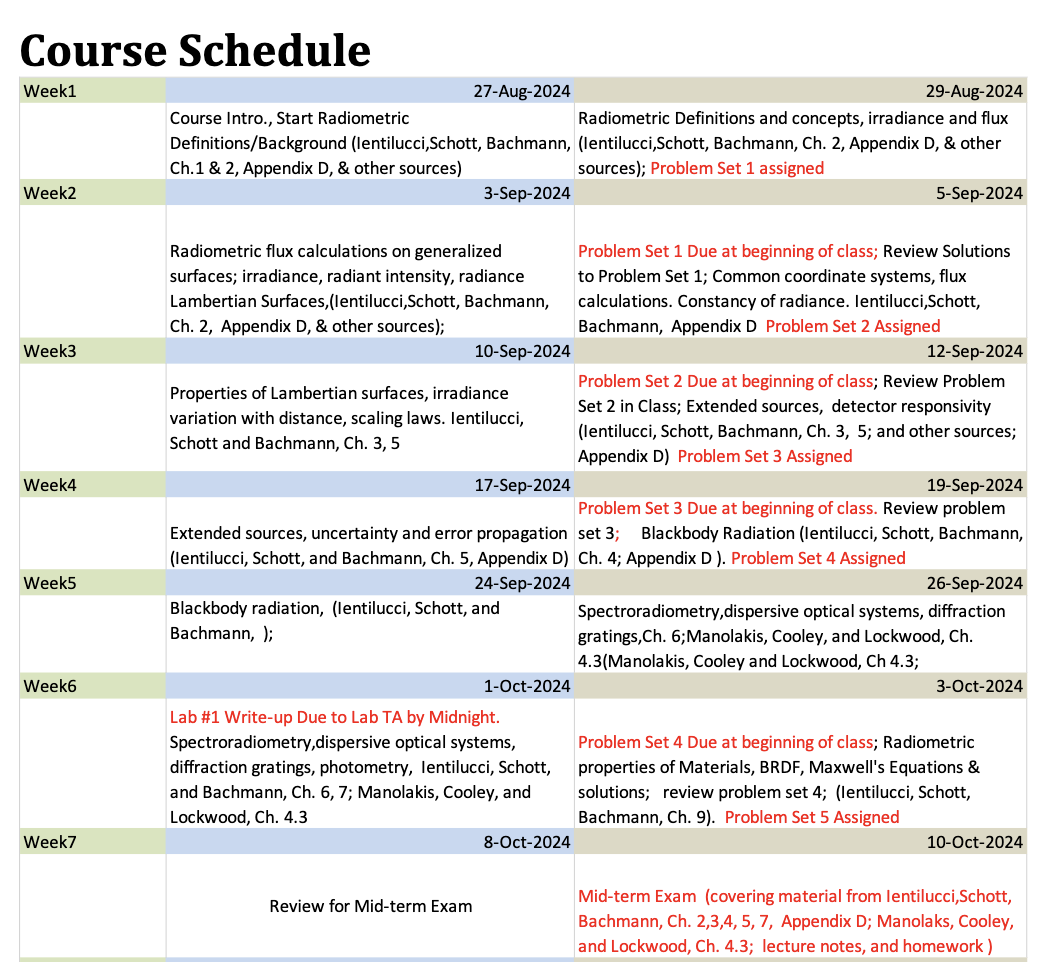
\includegraphics[scale=.95]{Radiometry/Week1/Notes/Syllabus.png}
%\caption{Course Syllabus: He goes through this pretty thoroughly, except that %we did not get to Week 6. The exam is on 2,3,4,5, and 6.}
%\label{fig:Snowman3}
%\end{figure}


\section{Equations}



%\subsection{The Grating Equation}
%Sometimes the given information is in number of grooves or lines per milimeter: lpm 
%$d_{mm} = \frac{1}{lpm}$
%\begin{equation}
%    \Gamma_{Tot}=d(sin \theta_{i} + sin \theta_{r}) = \frac{l}{N}(sin \theta_{i} + sin \theta_{r}) = m \lambda
%\end{equation}
%Where m =0,1,2,3,...

\section{HANA Tree and Marsh Study}
\clearpage
More pictures are available and in the repository of this LaTeX file. 
\begin{figure}[h!]
\centering
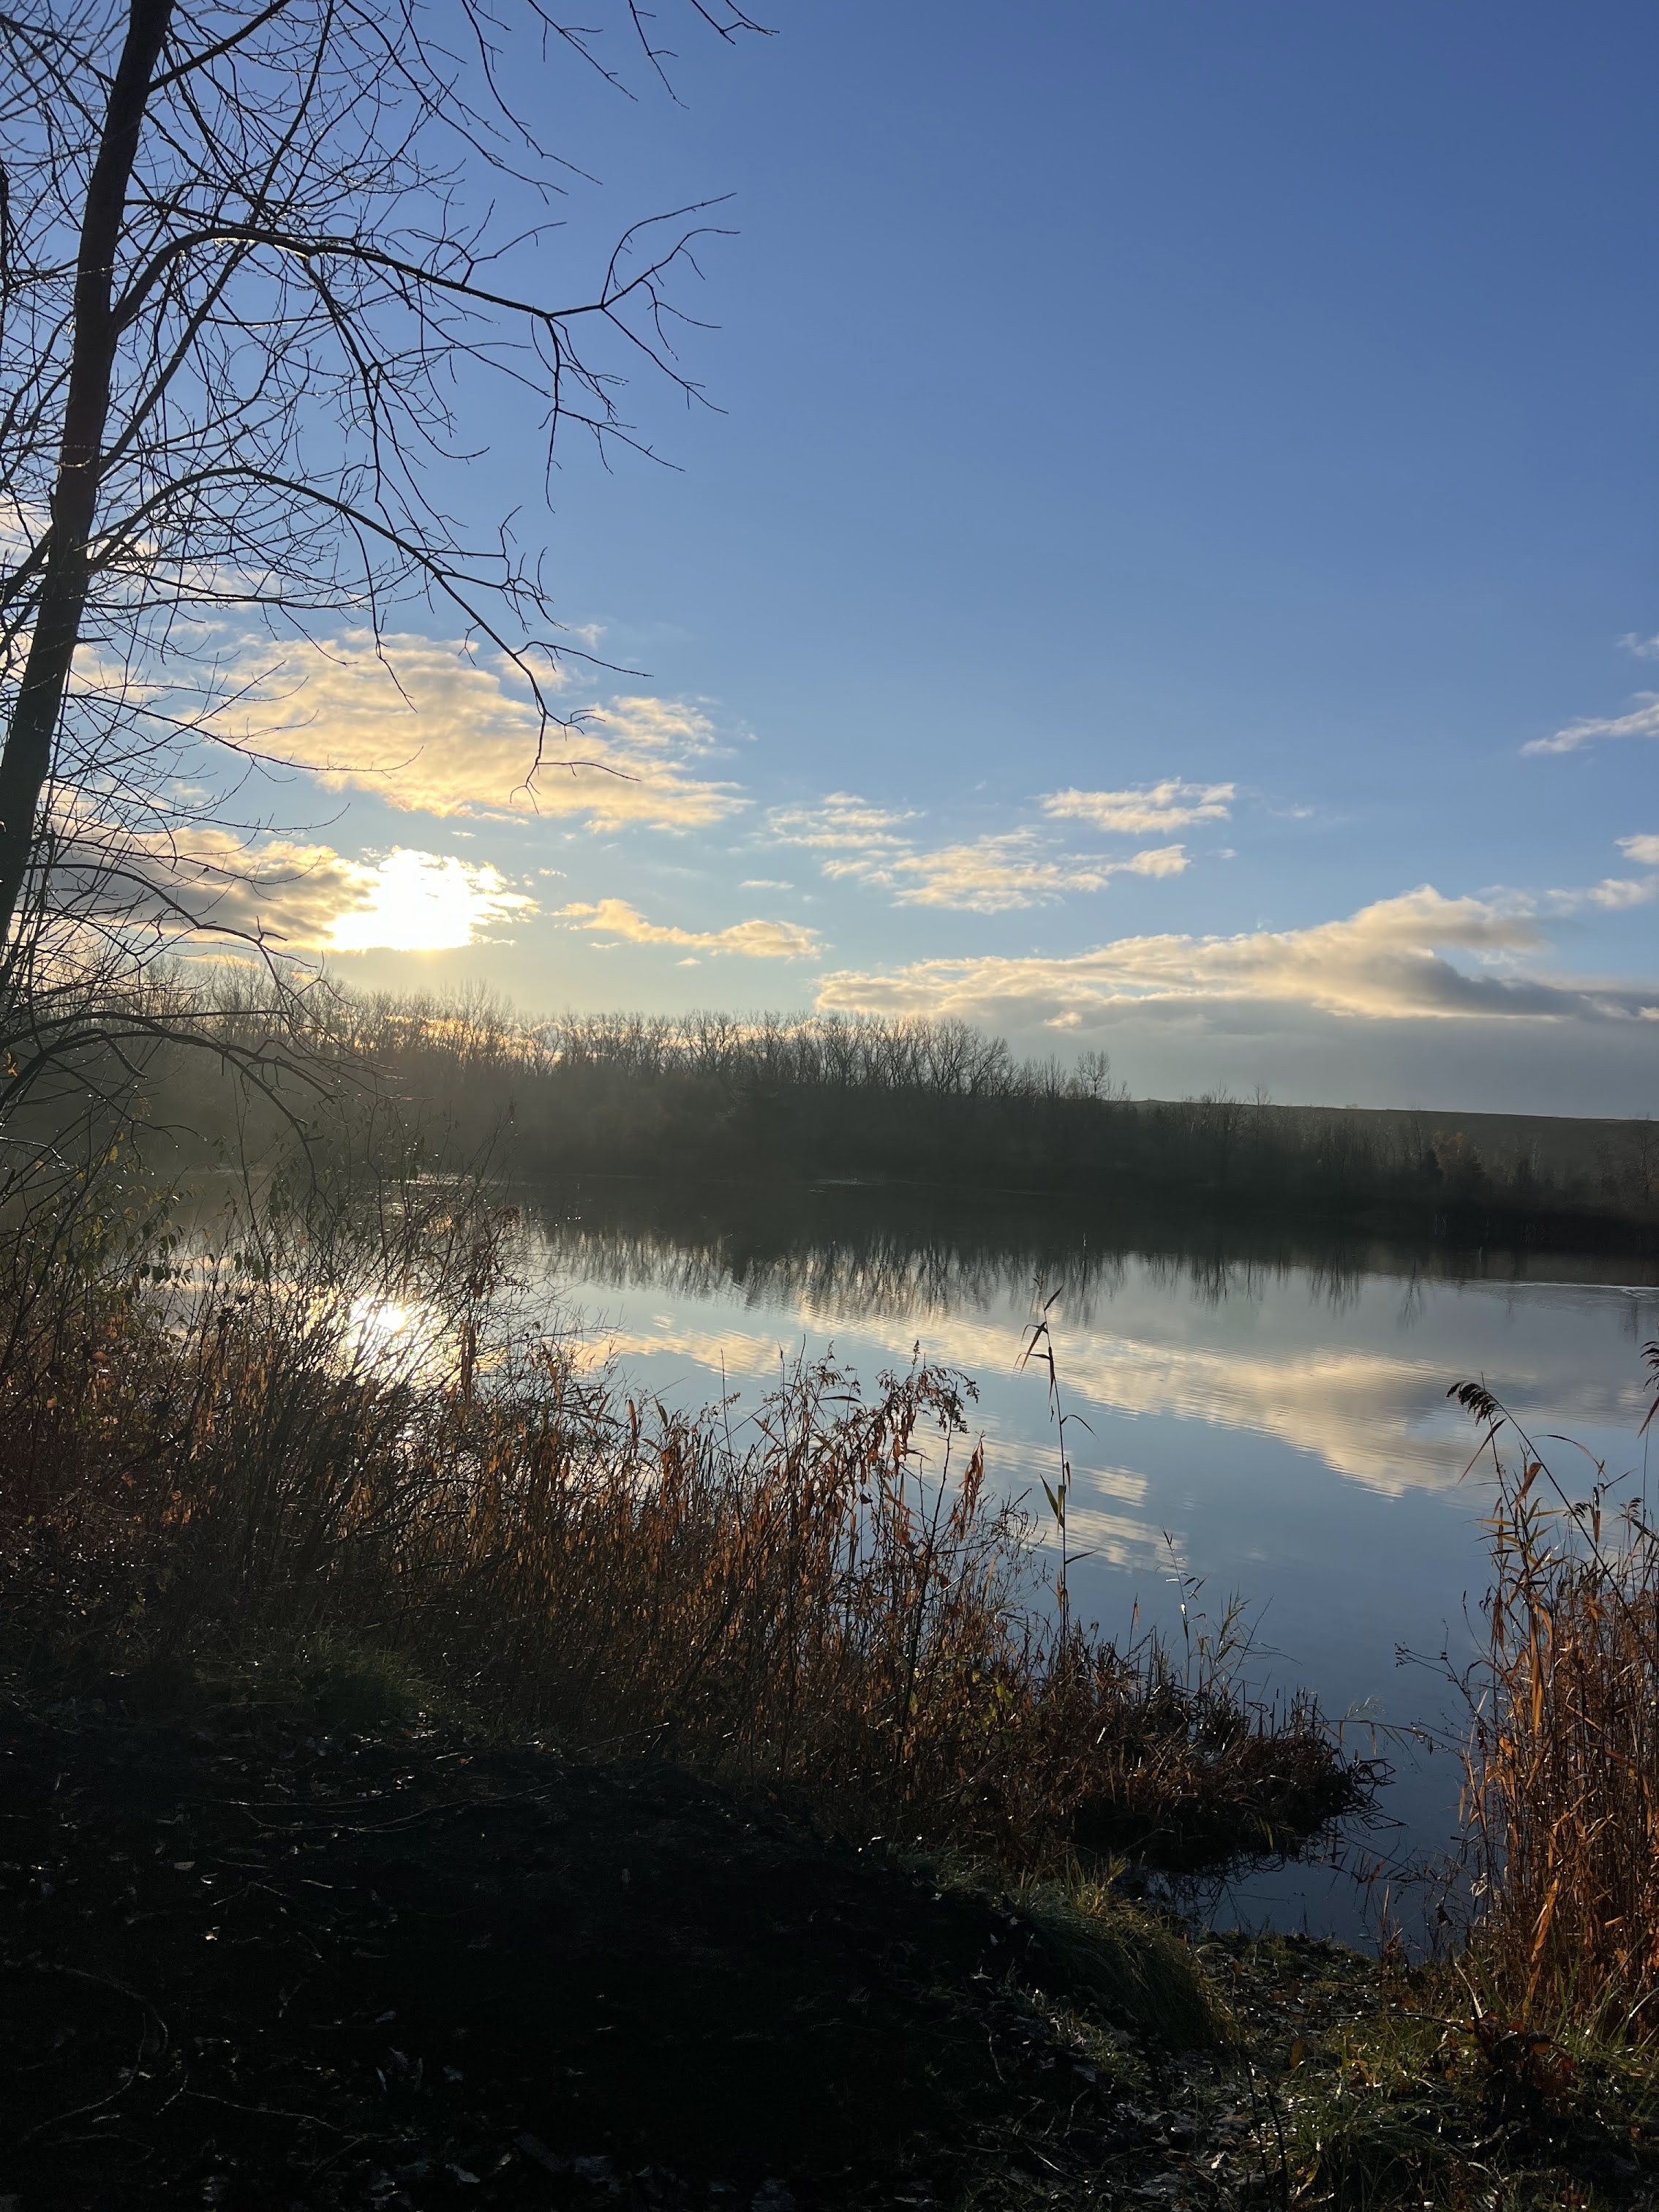
\includegraphics[scale=.1]{Research/HANA/NOV2024/IMG_9791.JPG}
\caption{HANA Tree Study}
\label{fig:HANA}
\end{figure}



\begin{figure}[h!]
\centering
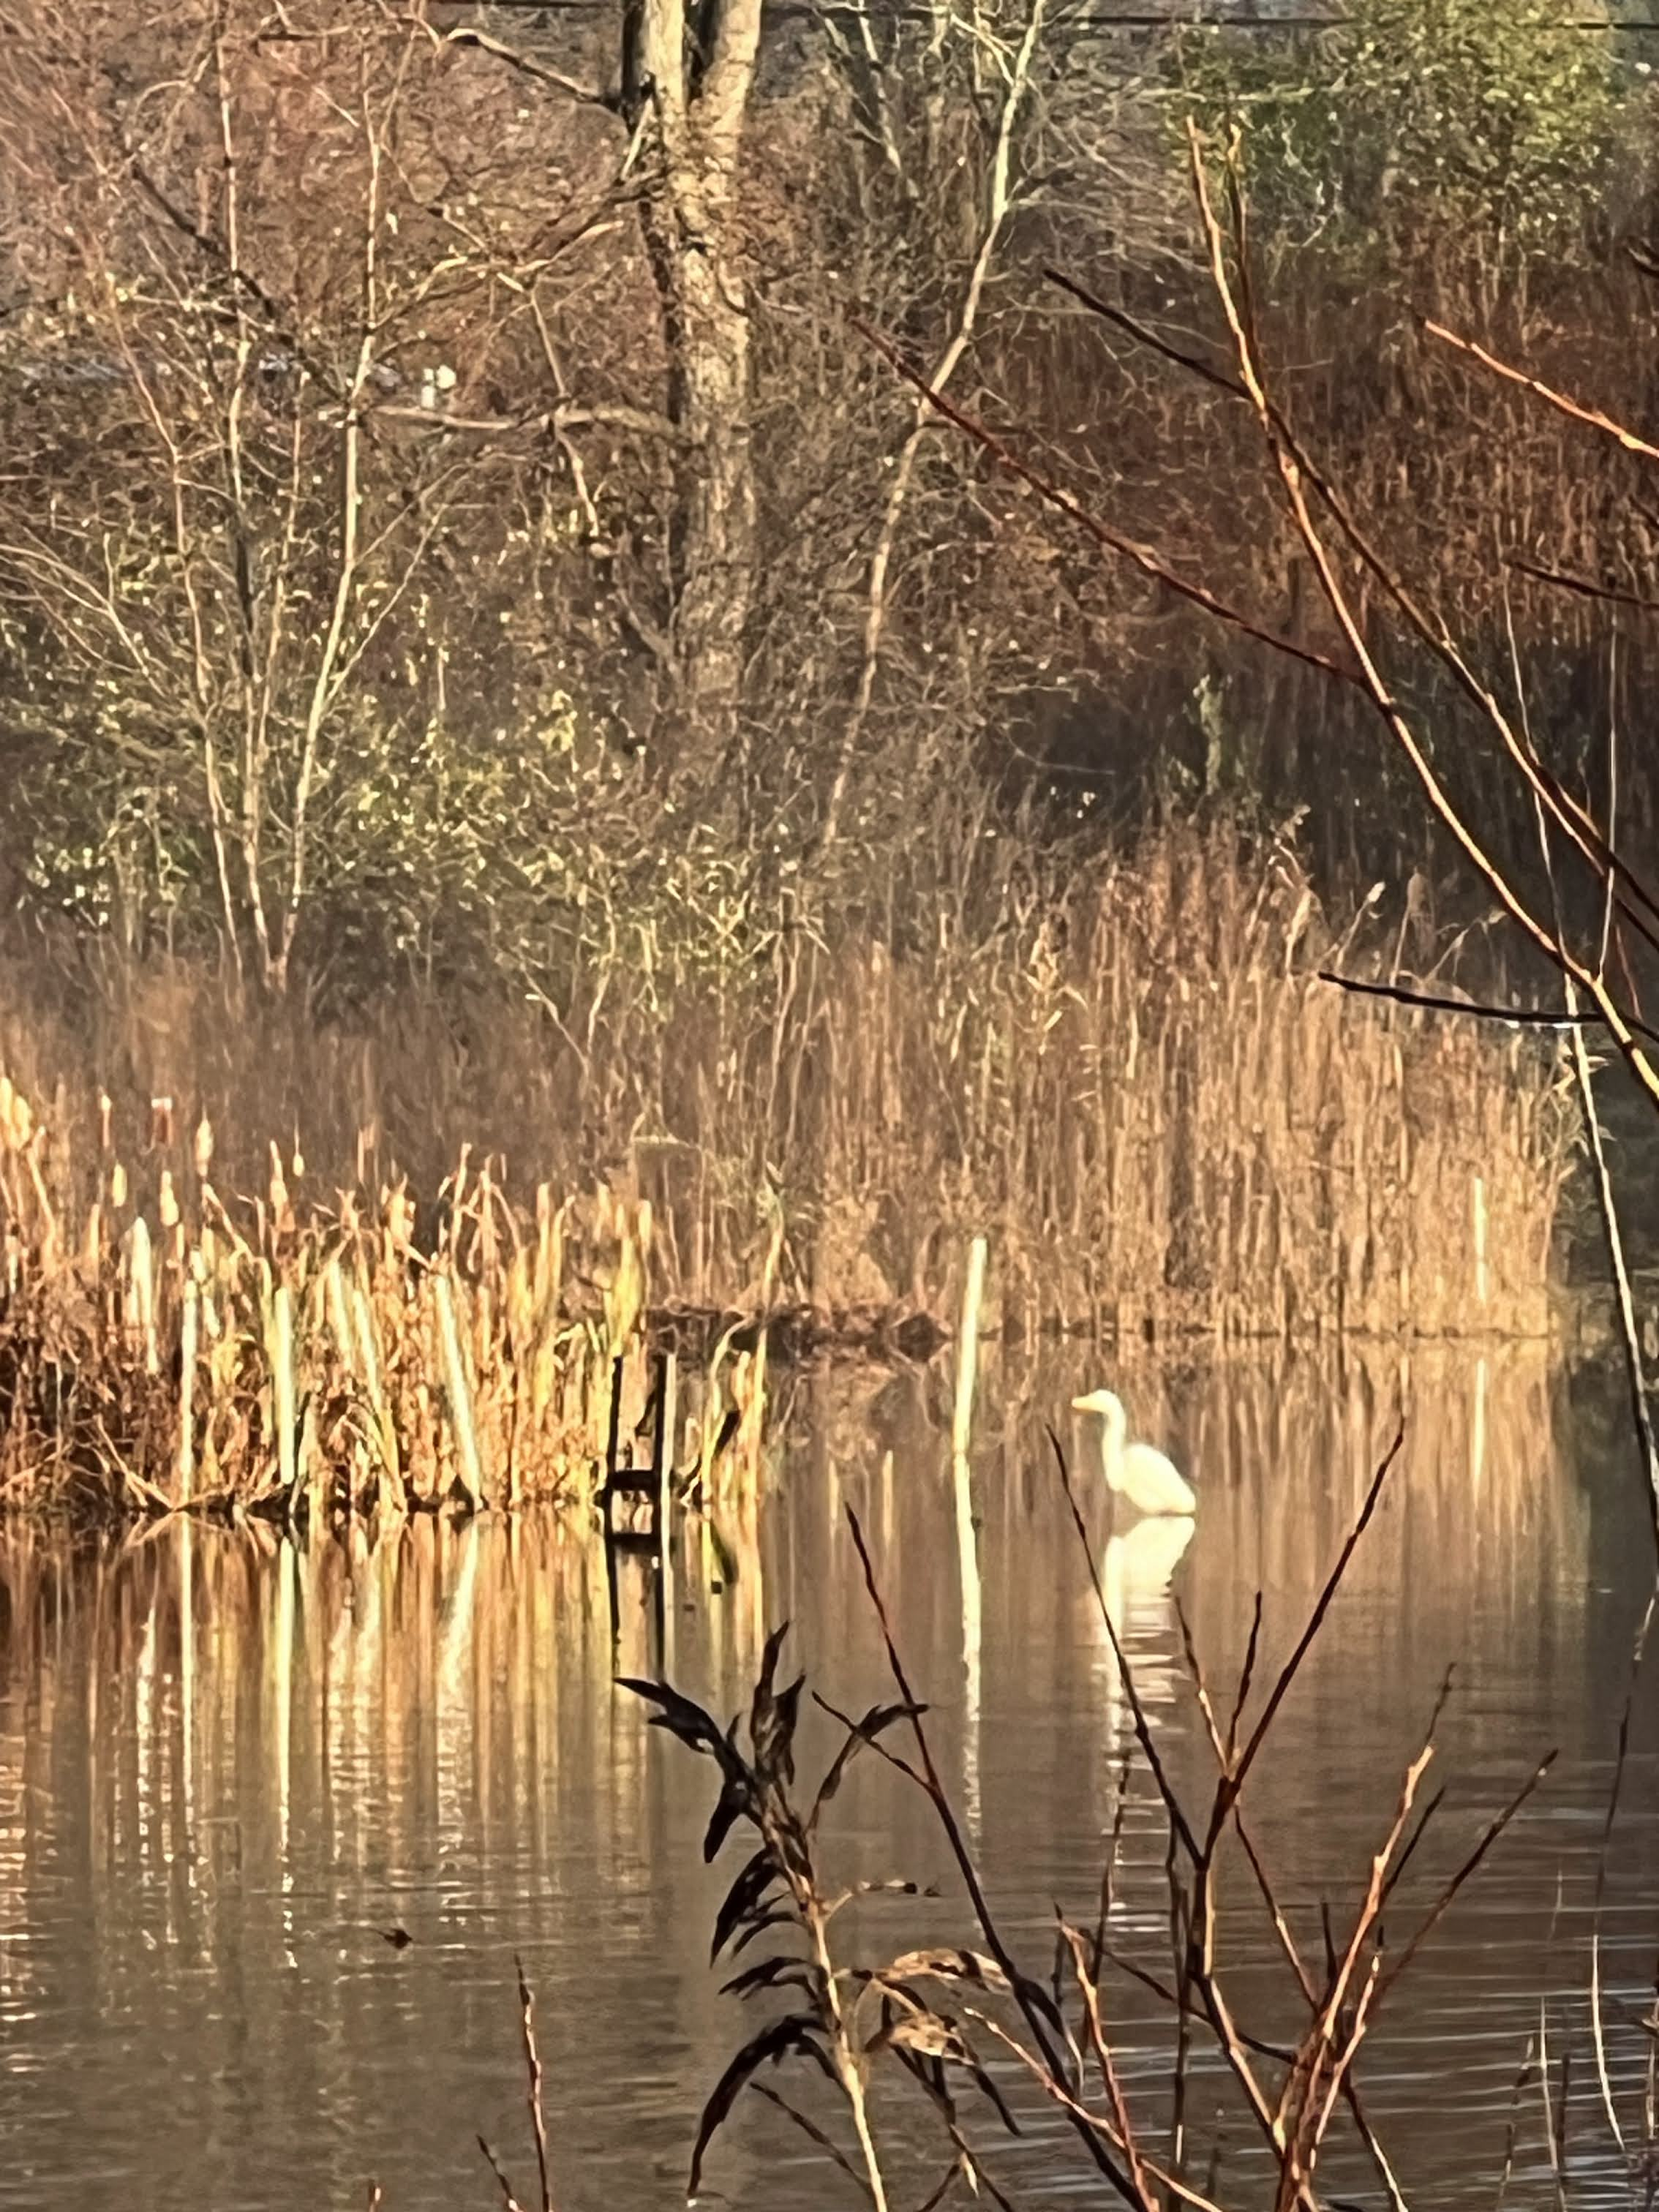
\includegraphics[scale=.1]{Research/HANA/NOV2024/IMG_9800.JPG}
\caption{HANA Tree Study}
\label{fig:HANA}
\end{figure}

\begin{figure}[h!]
\centering
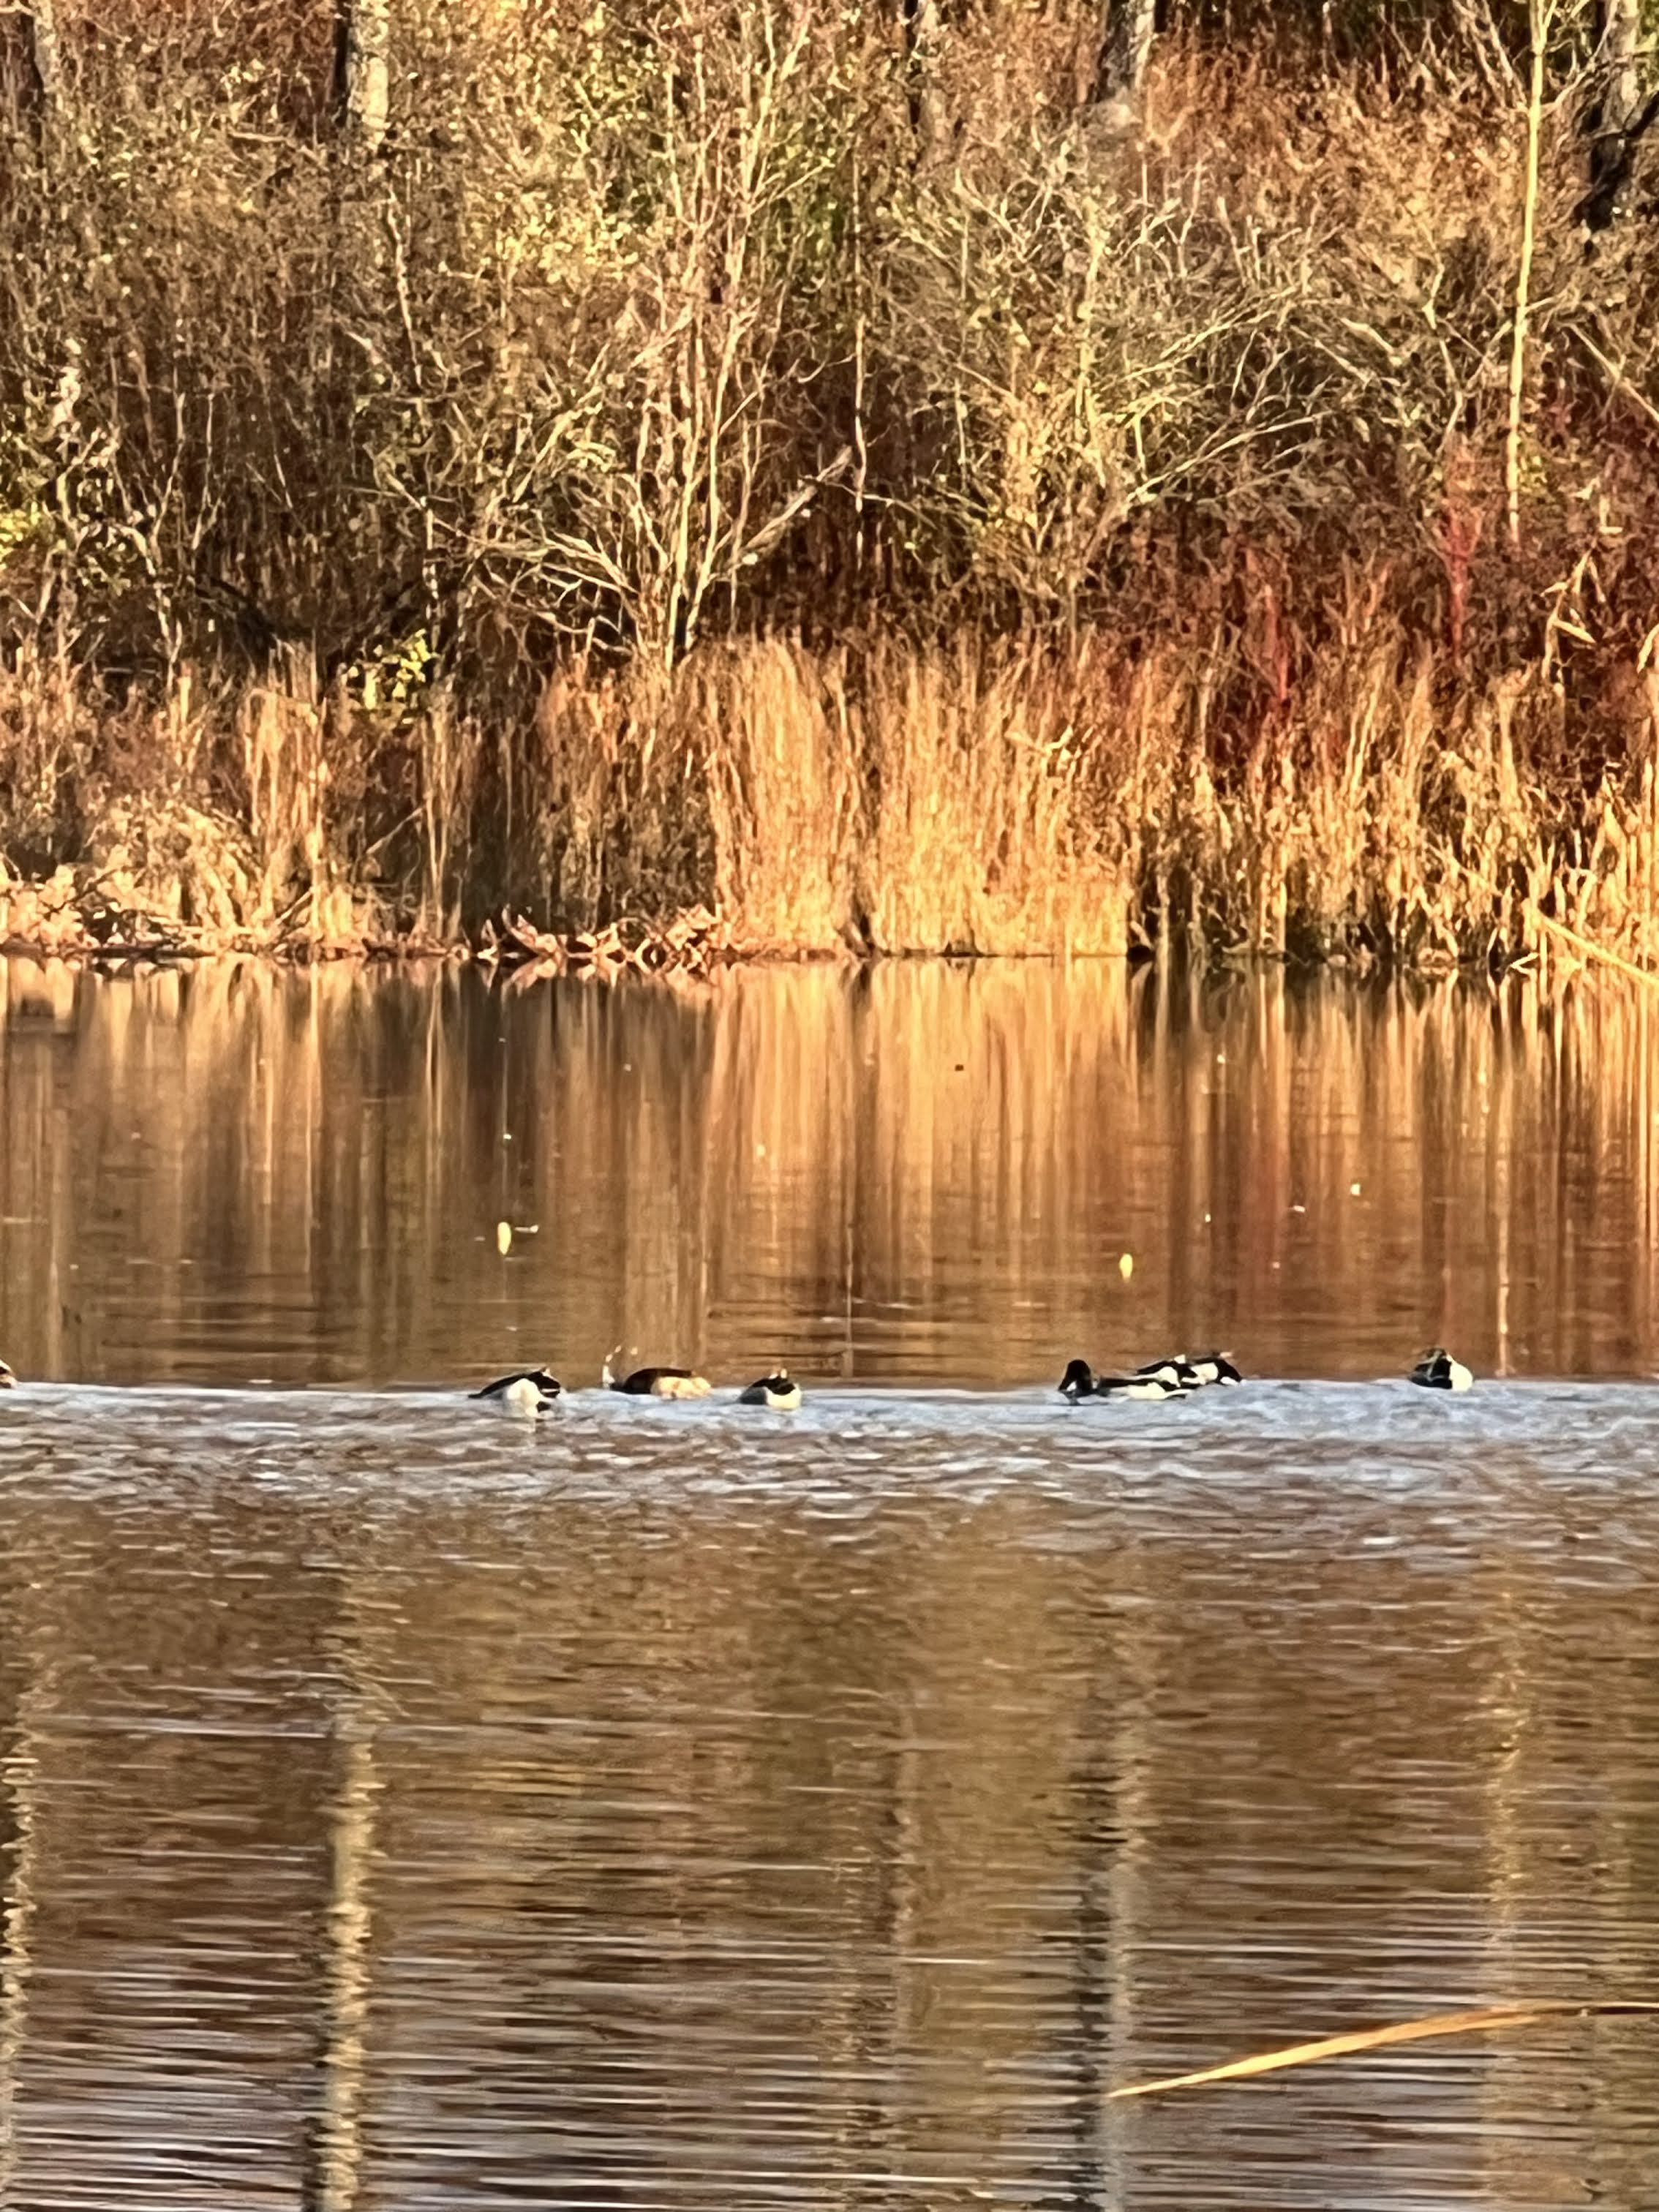
\includegraphics[scale=.1]{Research/HANA/NOV2024/IMG_9811.JPG}
\caption{HANA Tree Study}
\label{fig:HANA}
\end{figure}

\begin{figure}[h!]
\centering
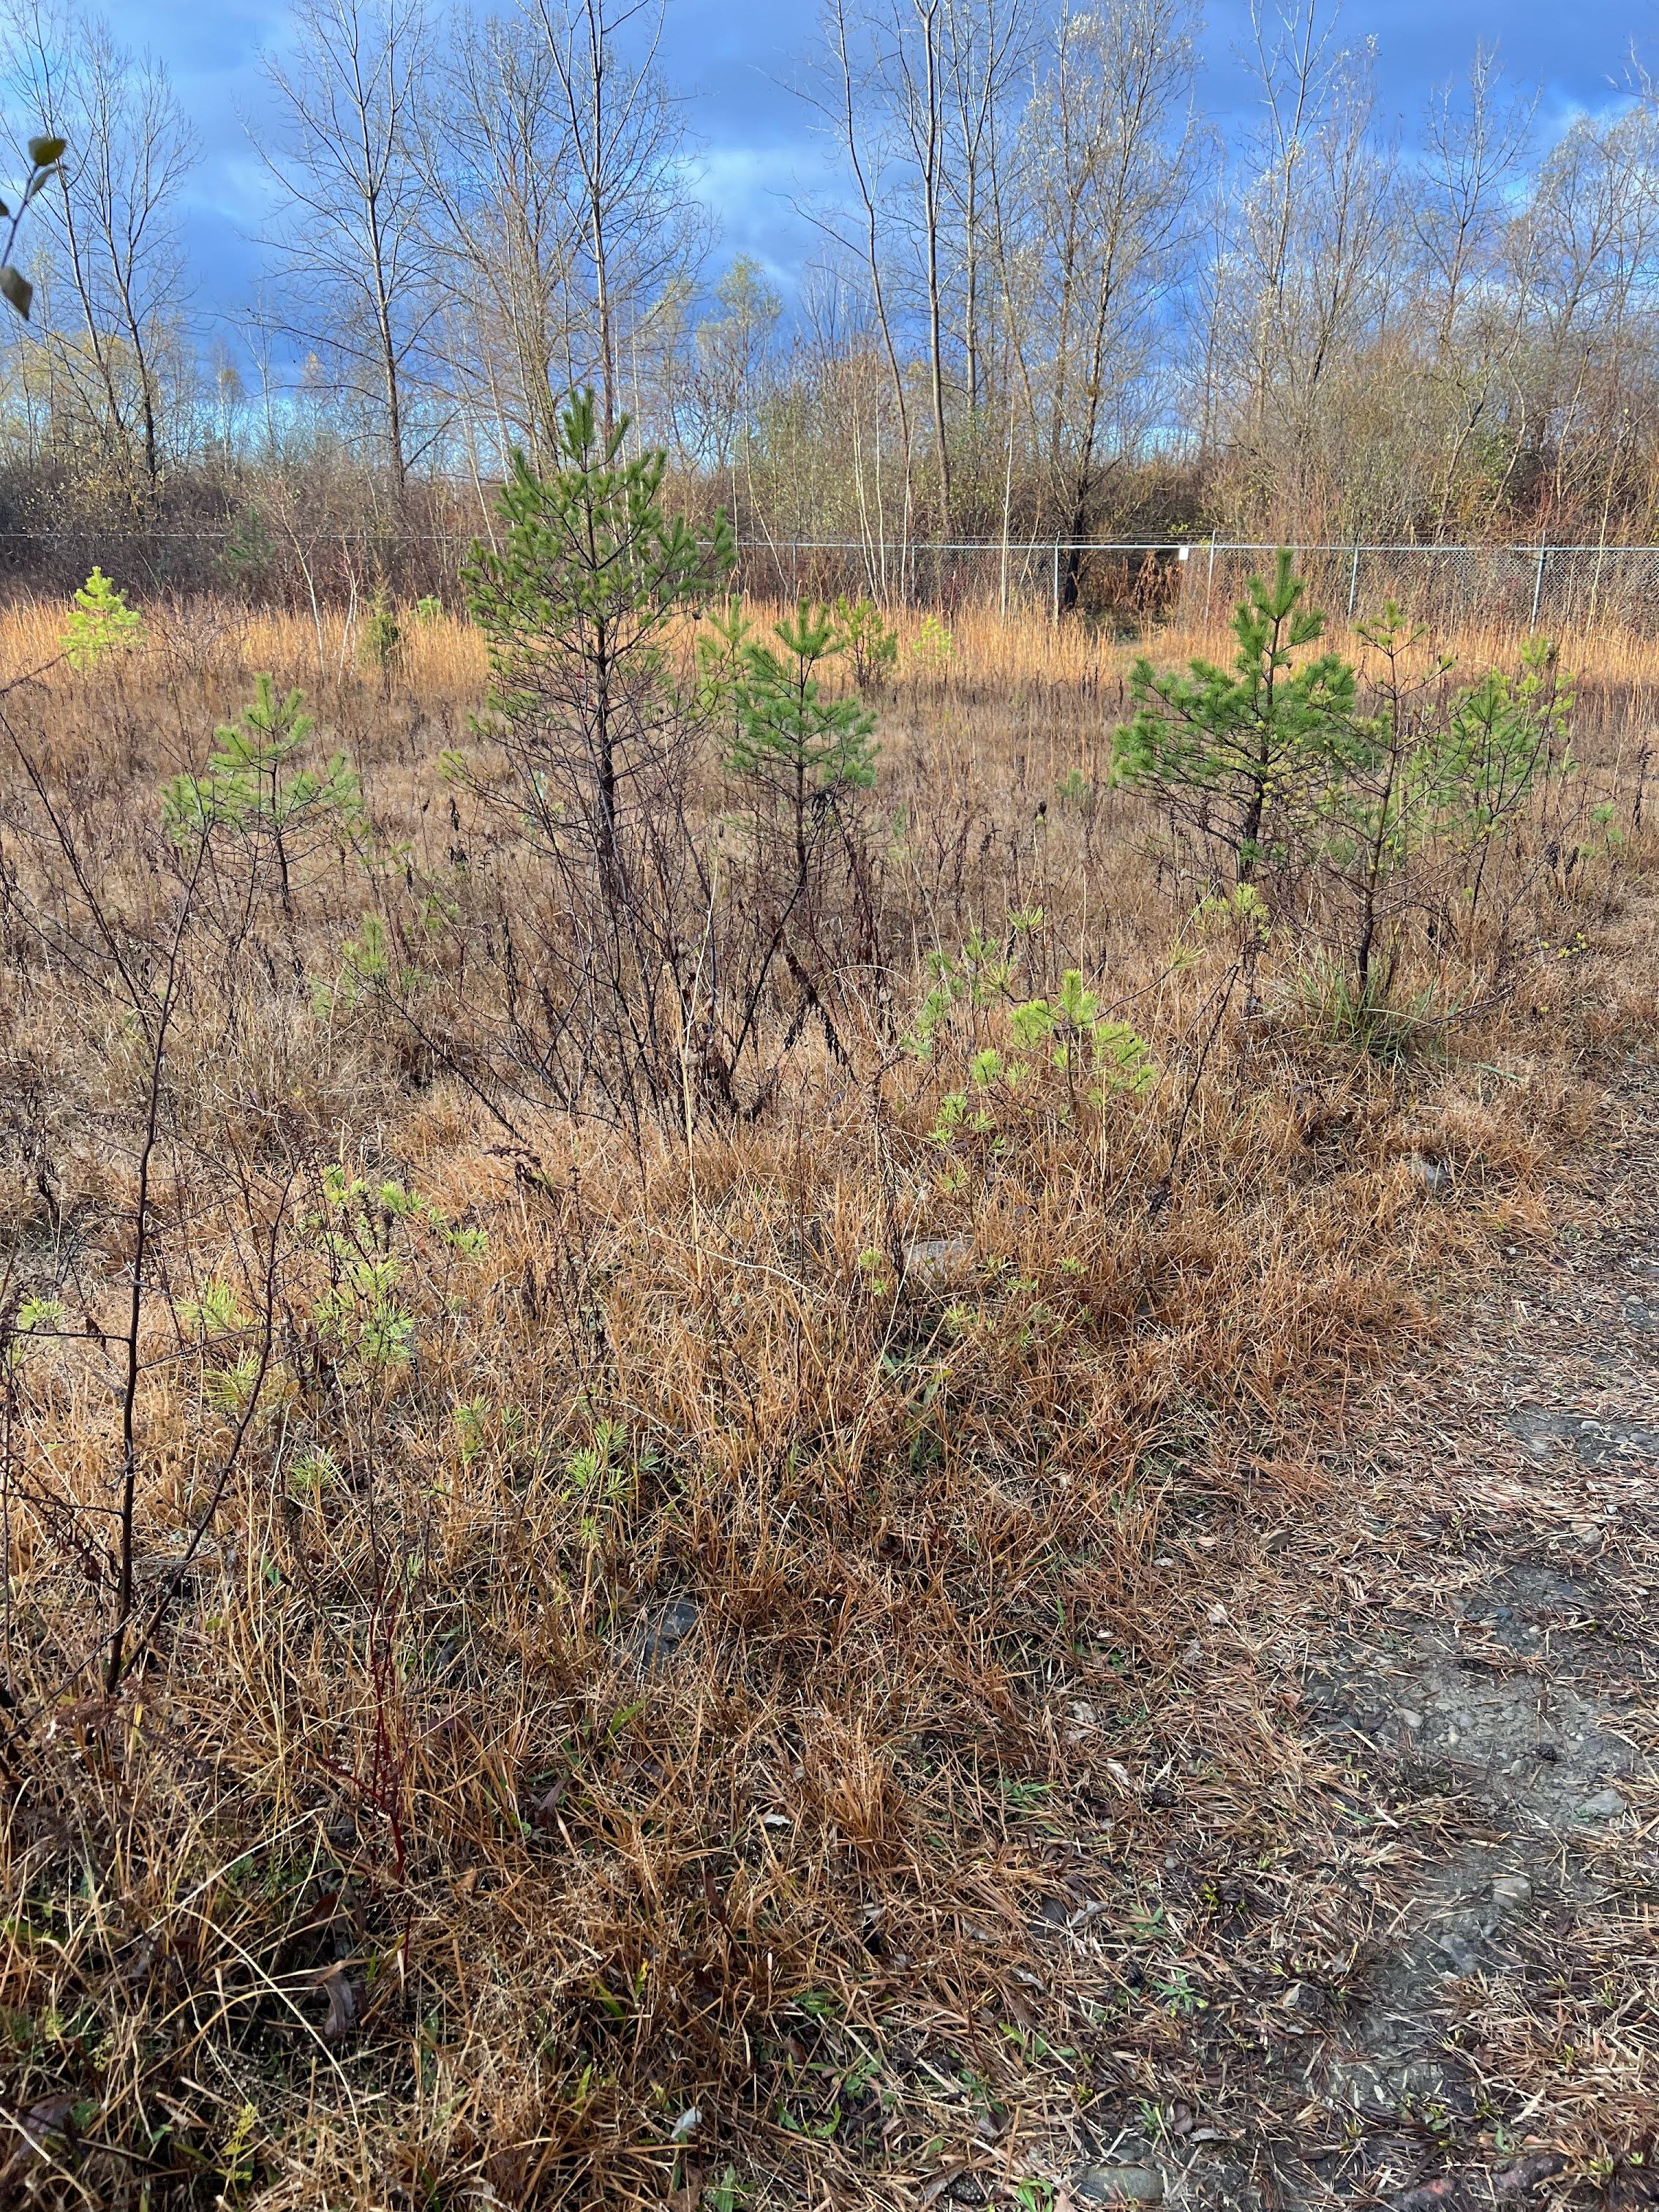
\includegraphics[scale=.1]{Research/HANA/NOV2024/IMG_9820.JPG}
\caption{HANA Tree Study}
\label{fig:HANA}
\end{figure}

\begin{figure}[h!]
\centering
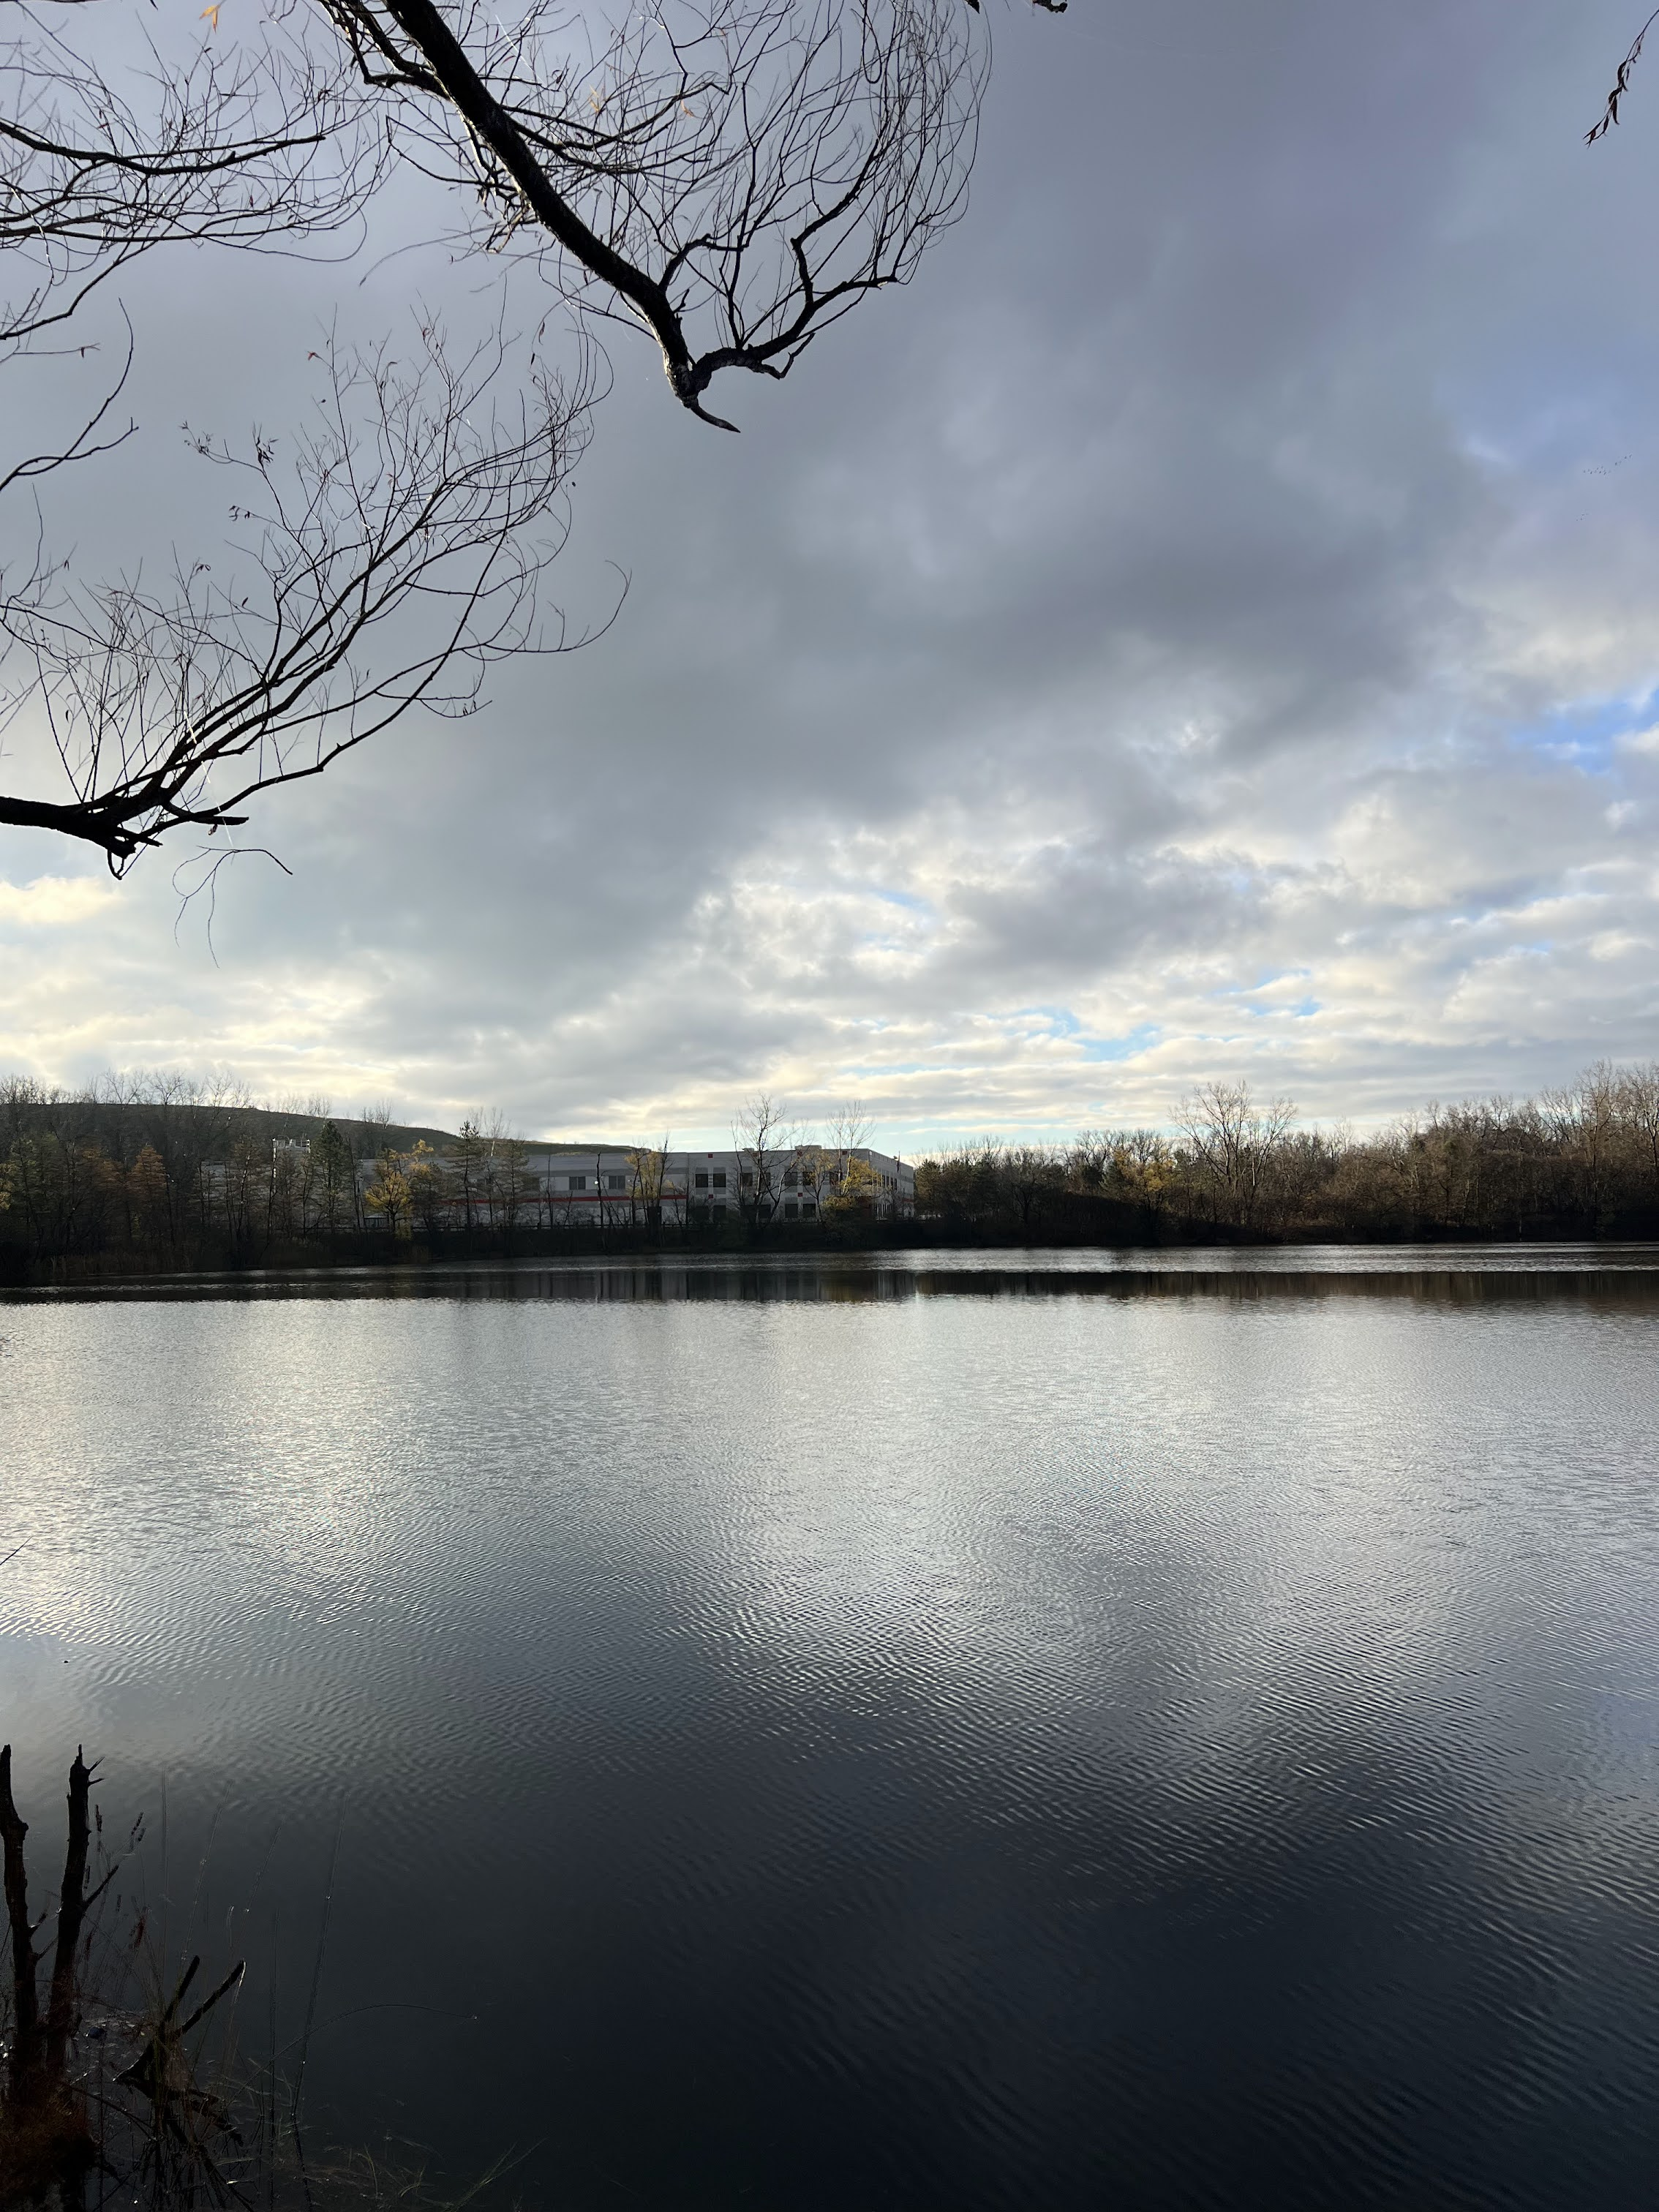
\includegraphics[scale=.1]{Research/HANA/NOV2024/IMG_9830.JPG}
\caption{HANA Tree Study}
\label{fig:HANA}
\end{figure}

\begin{figure}[h!]
\centering
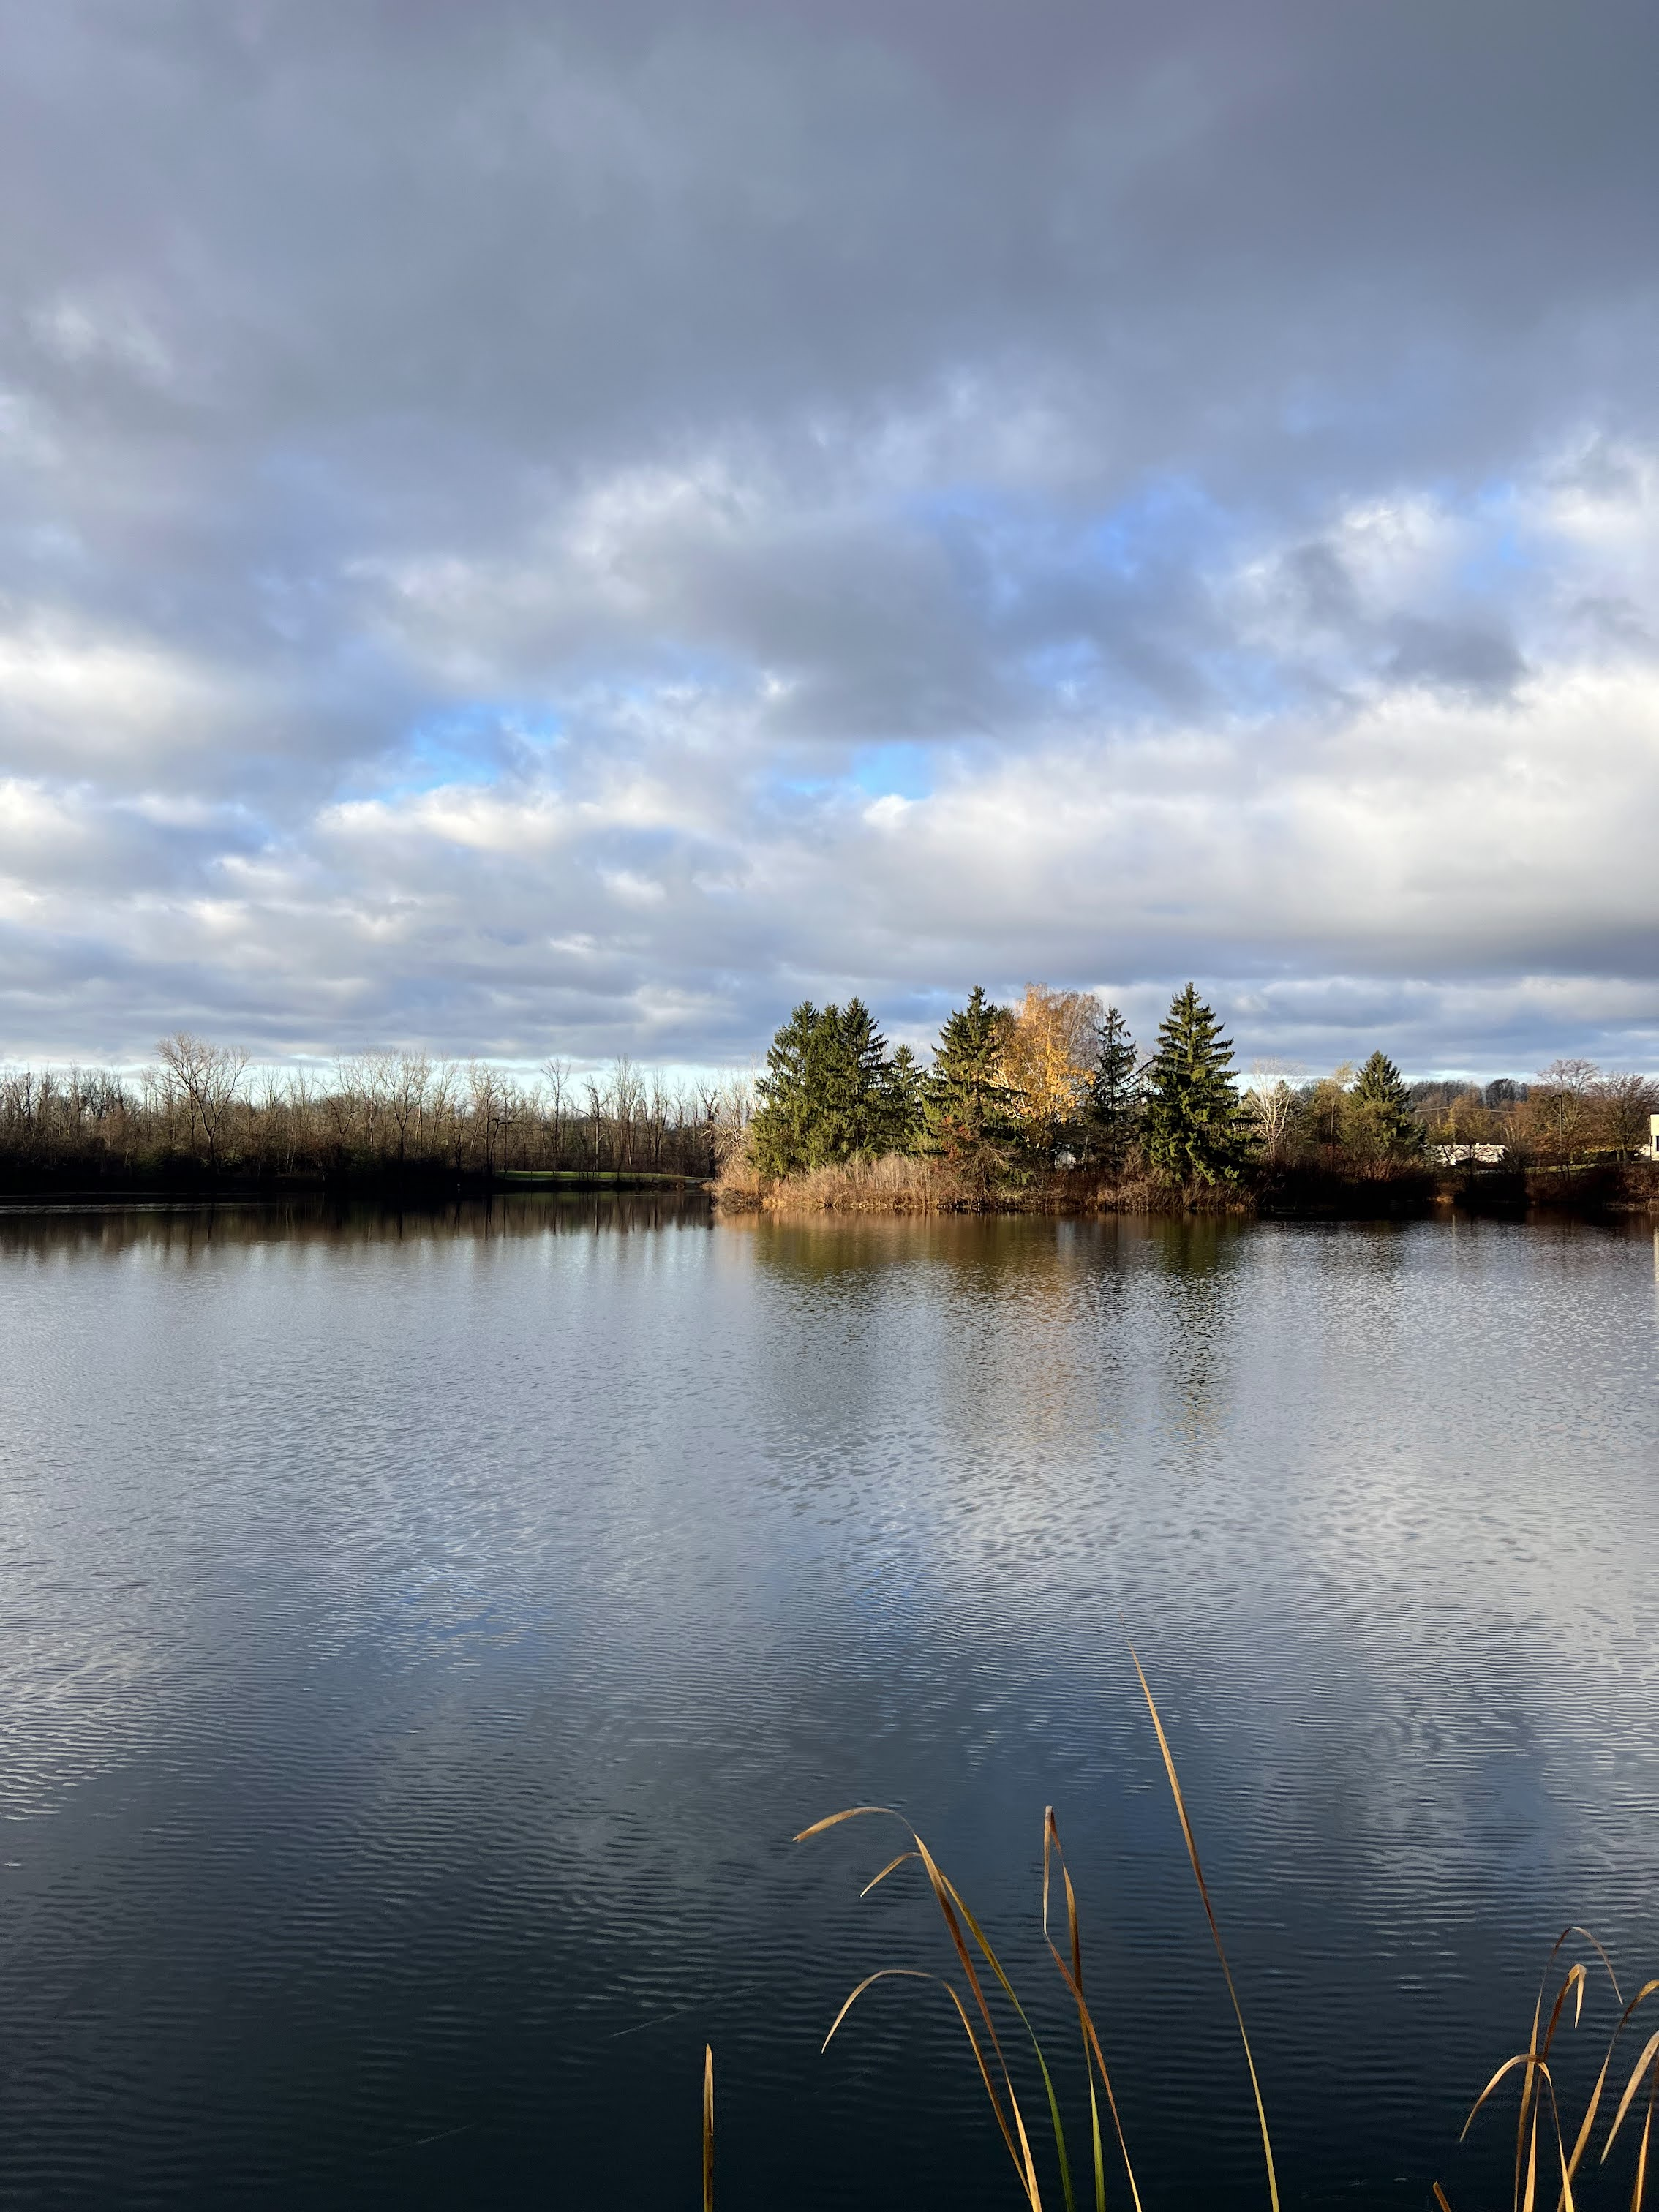
\includegraphics[scale=.1]{Research/HANA/NOV2024/IMG_9834.JPG}
\caption{HANA Tree Study}
\label{fig:HANA}
\end{figure}

\begin{figure}[h!]
\centering
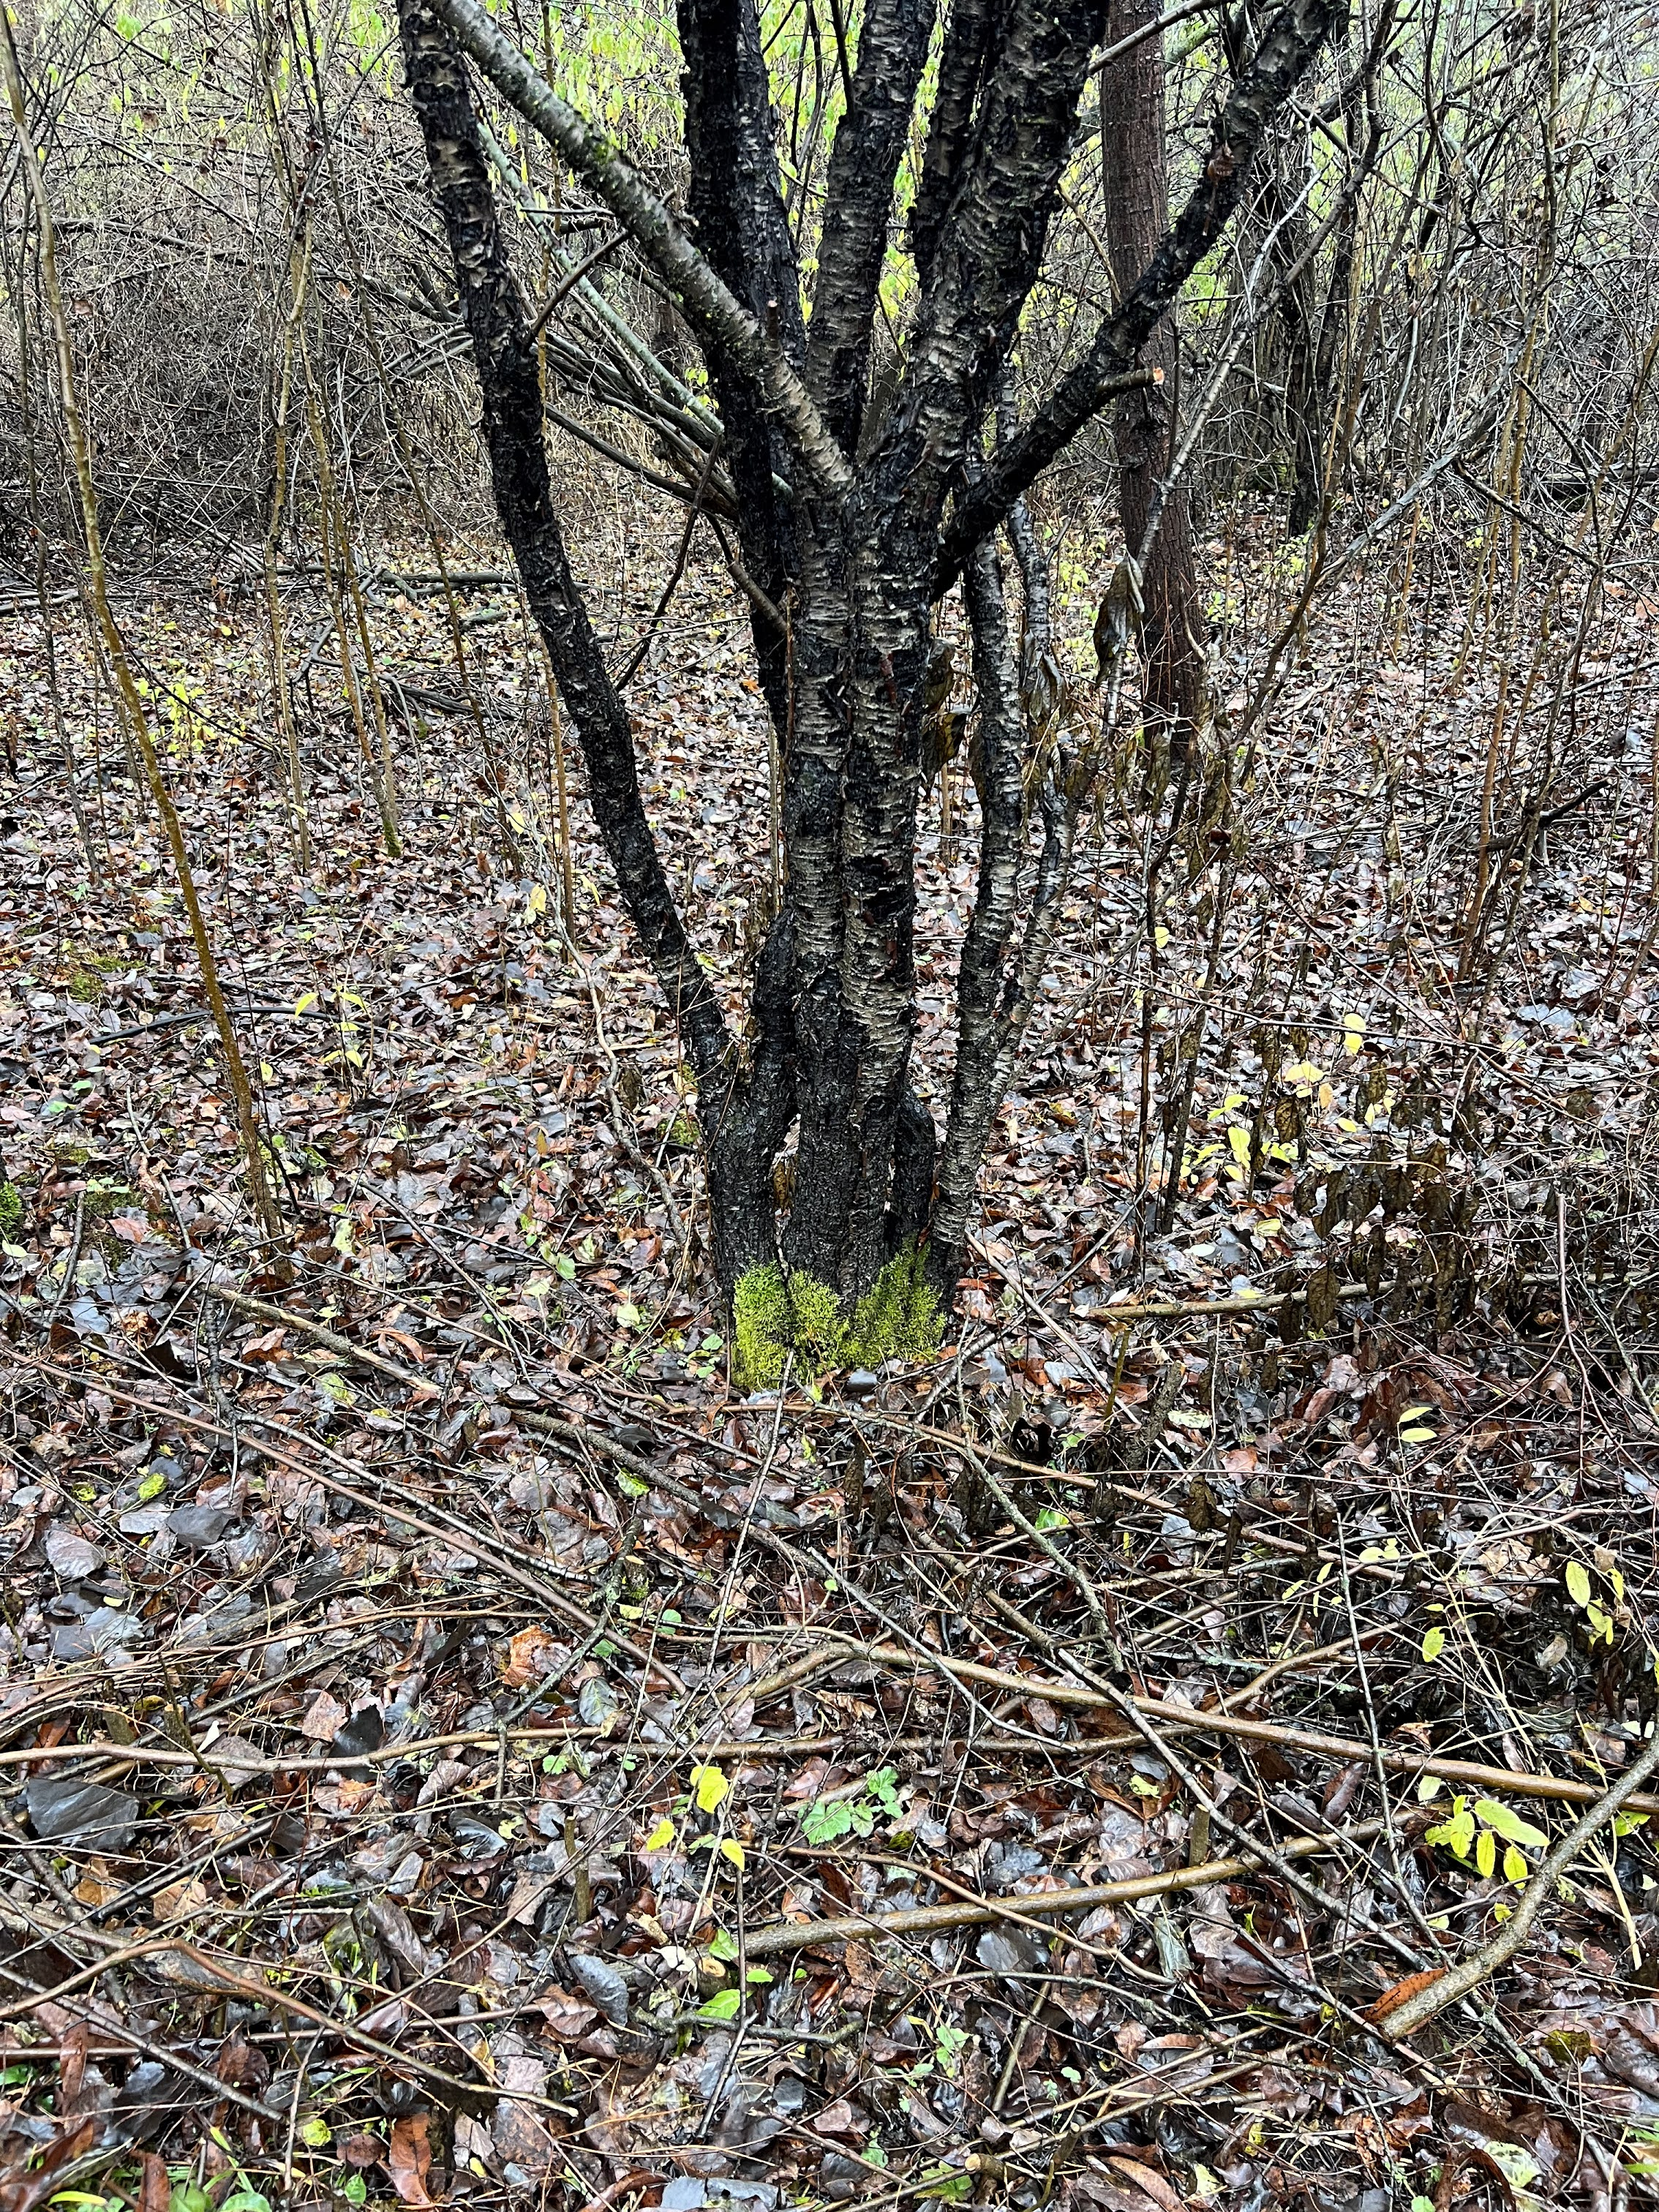
\includegraphics[scale=.1]{Research/HANA/NOV2024/IMG_9845.JPG}
\caption{HANA Tree Study}
\label{fig:HANA}
\end{figure}



\begin{figure}[h!]
\centering
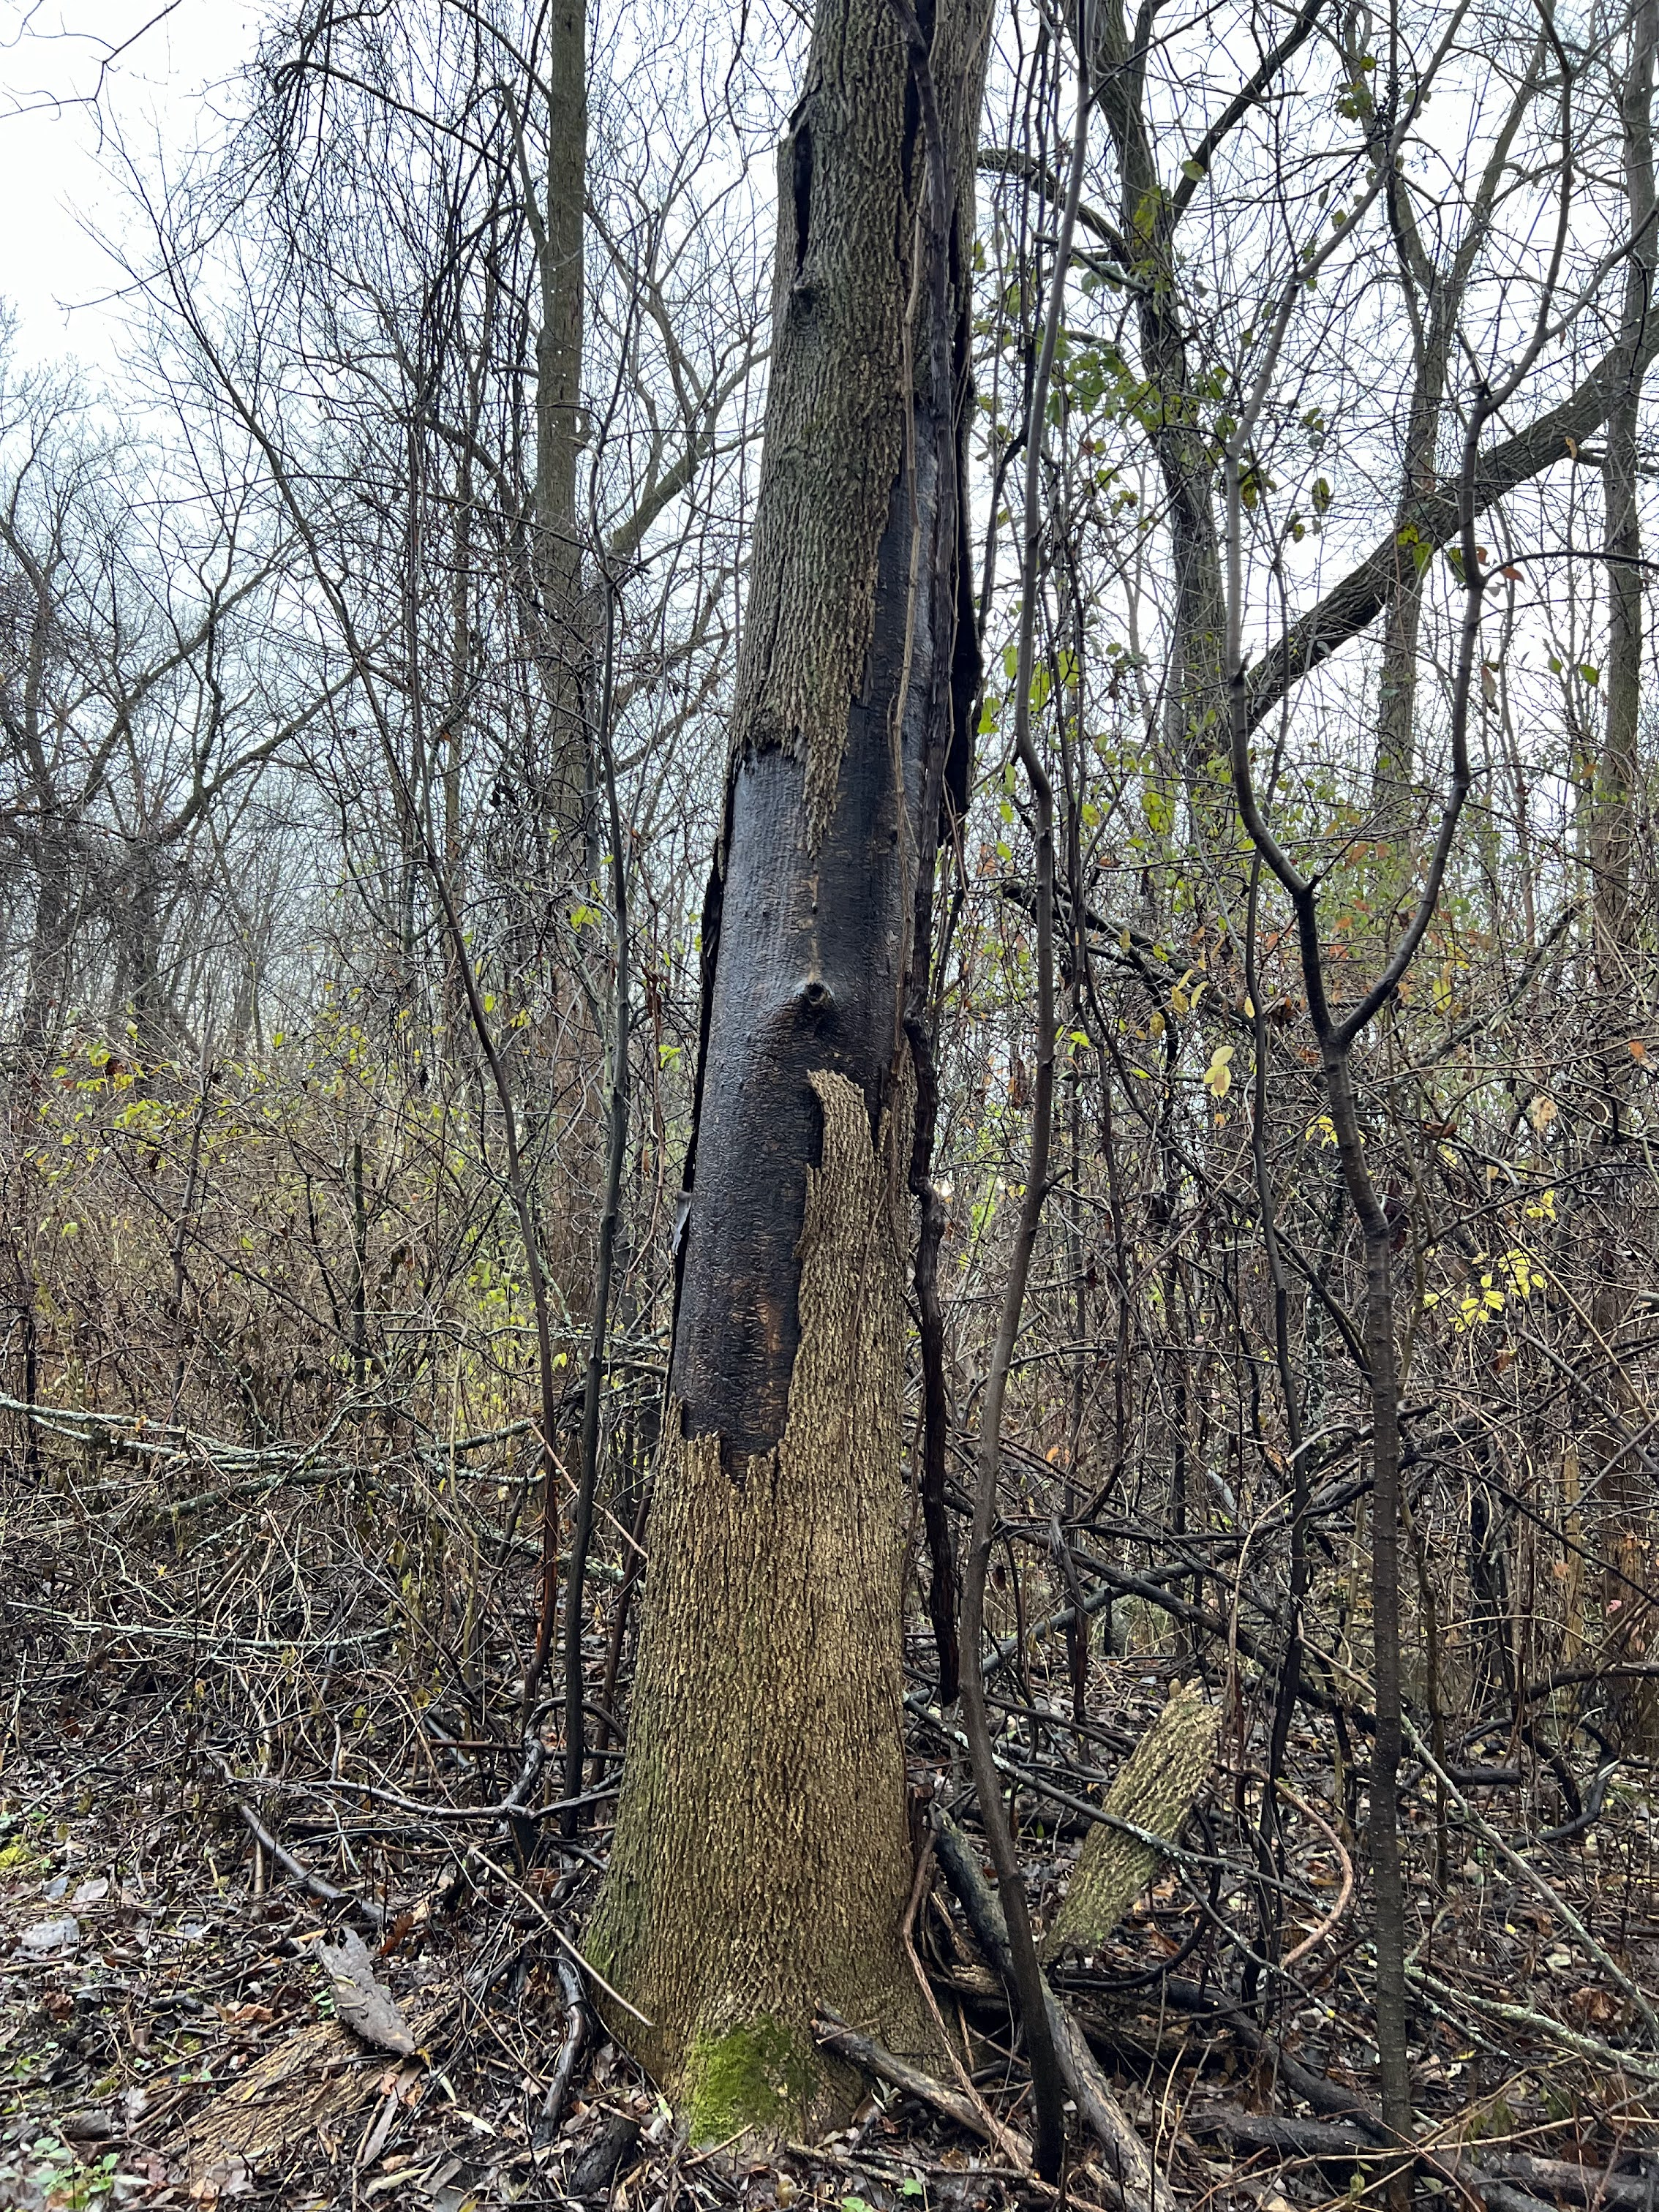
\includegraphics[scale=.1]{Research/HANA/NOV2024/IMG_9848.JPG}
\caption{HANA Tree Study}
\label{fig:HANA}
\end{figure}


\begin{figure}[h!]
\centering
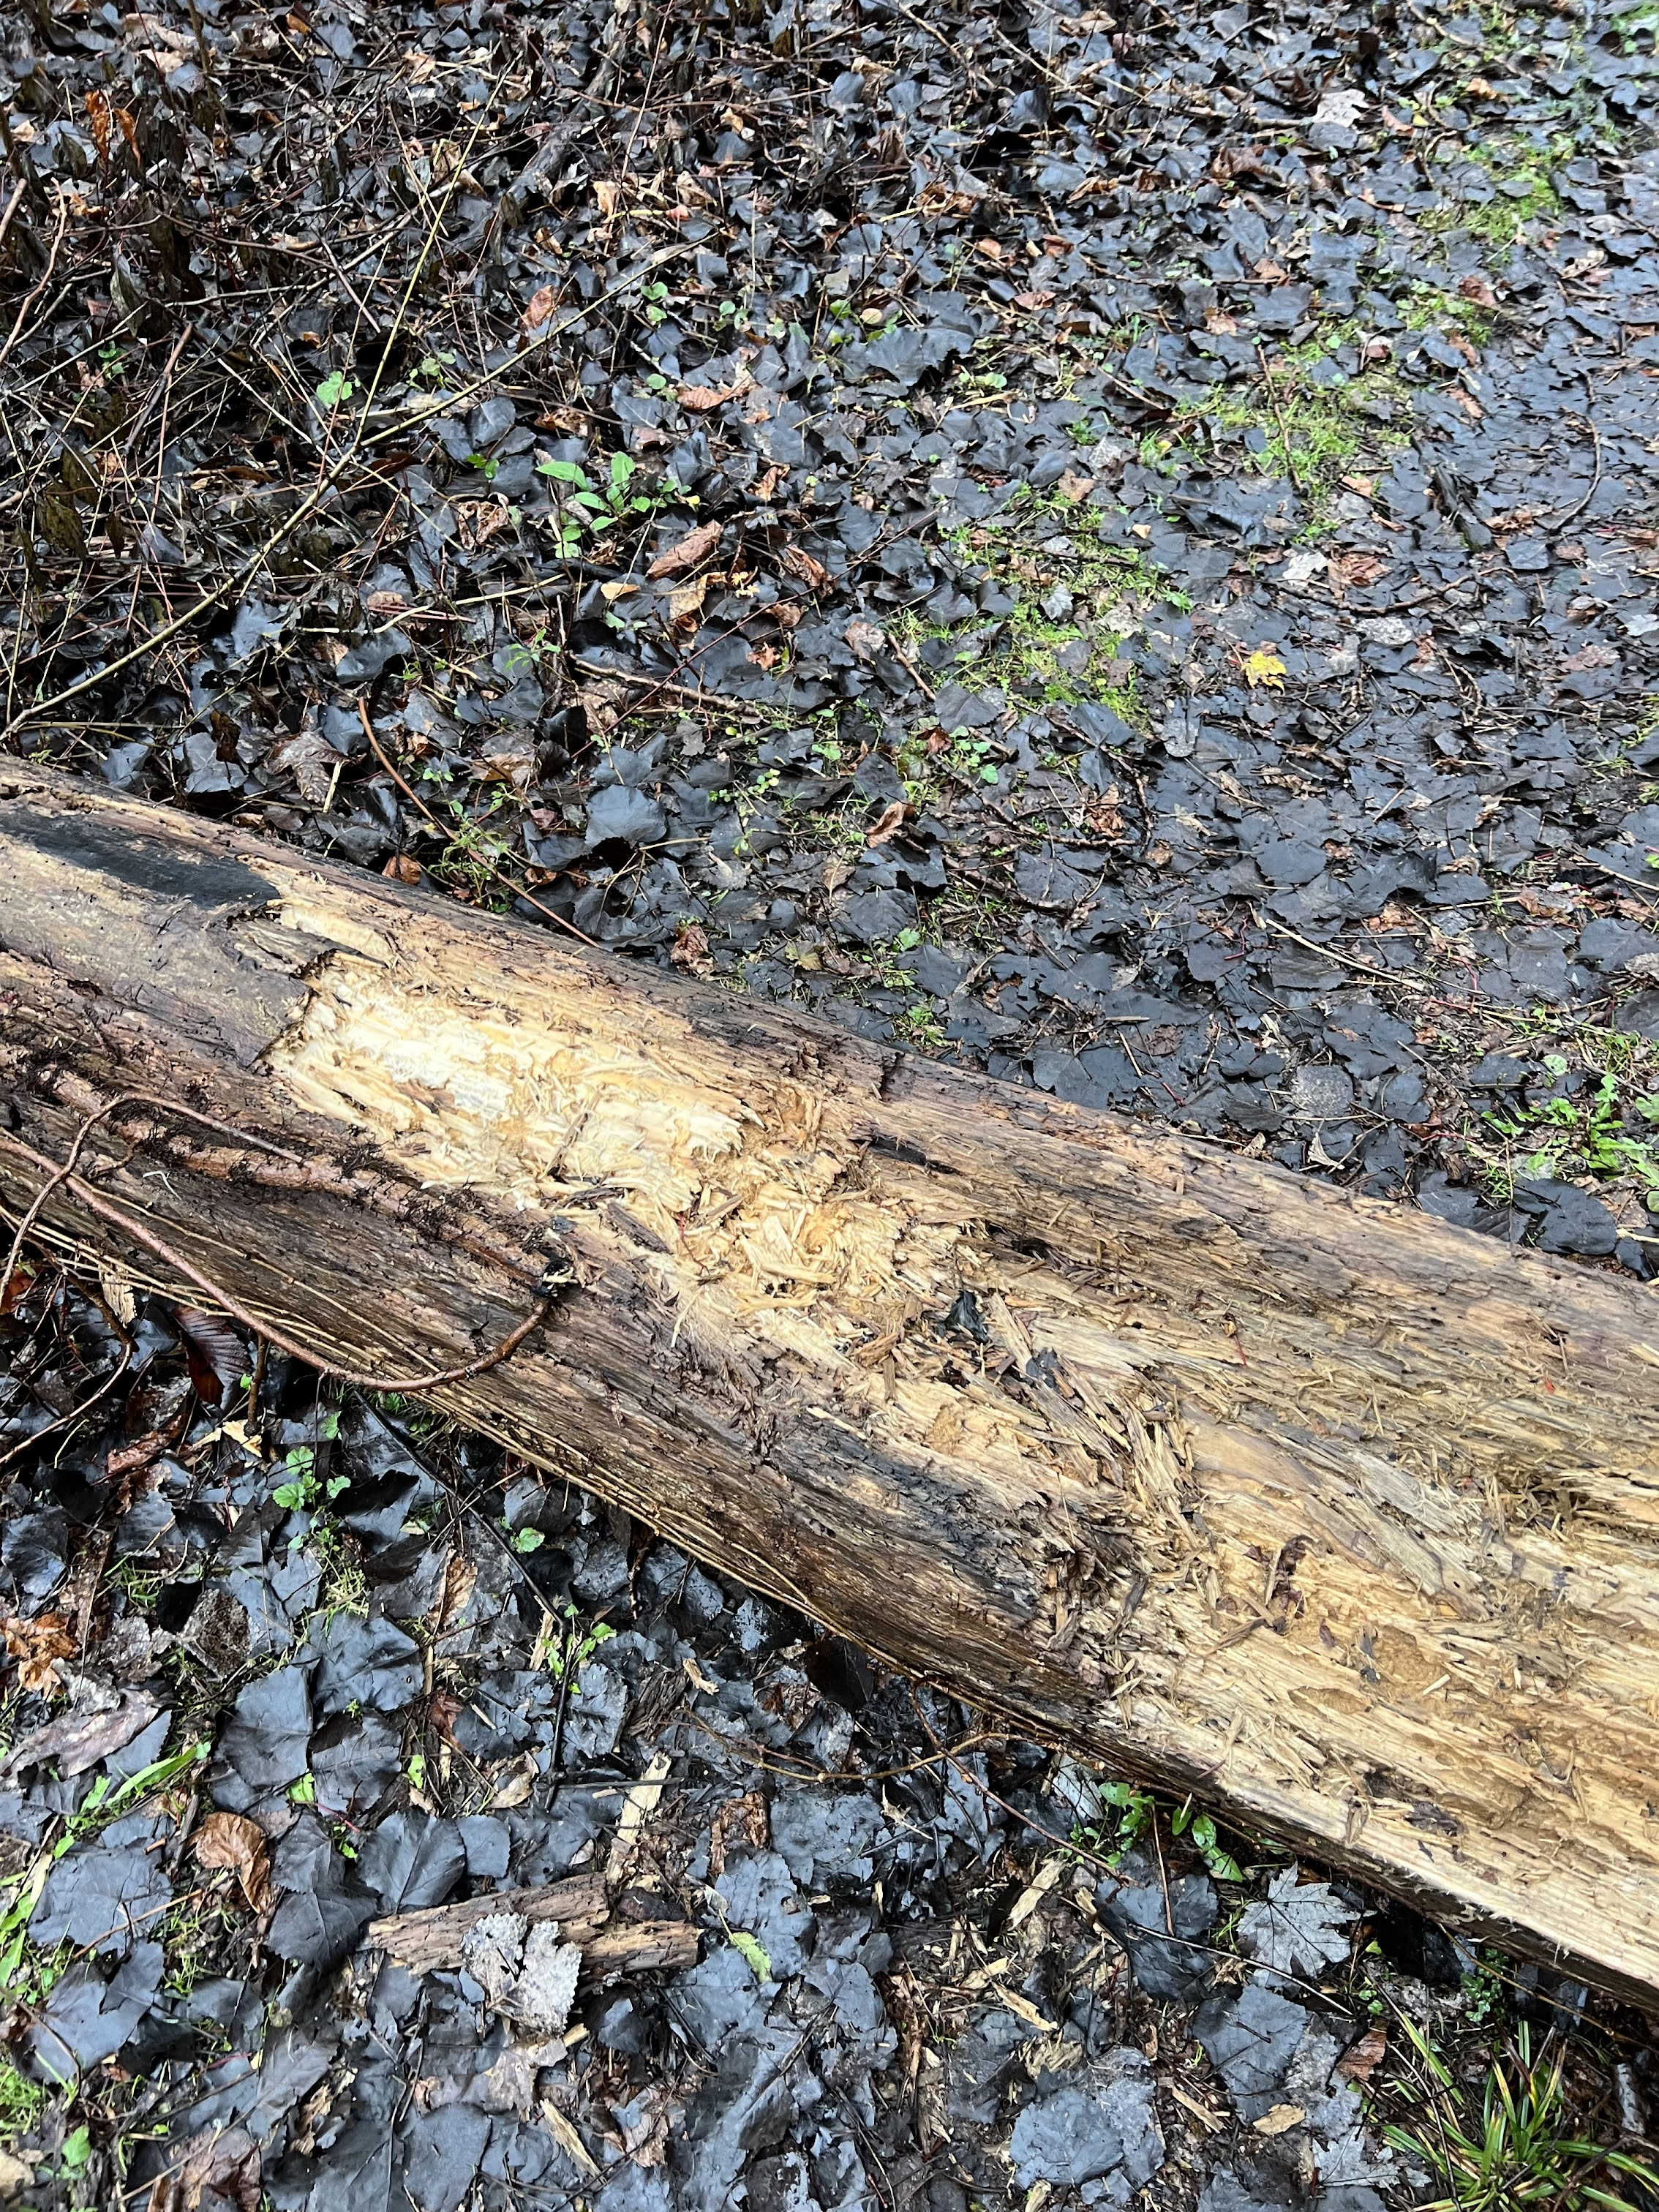
\includegraphics[scale=.1]{Research/HANA/NOV2024/IMG_9852.JPG}
\caption{HANA Tree Study}
\label{fig:HANA}
\end{figure}



\begin{figure}[h!]
\centering
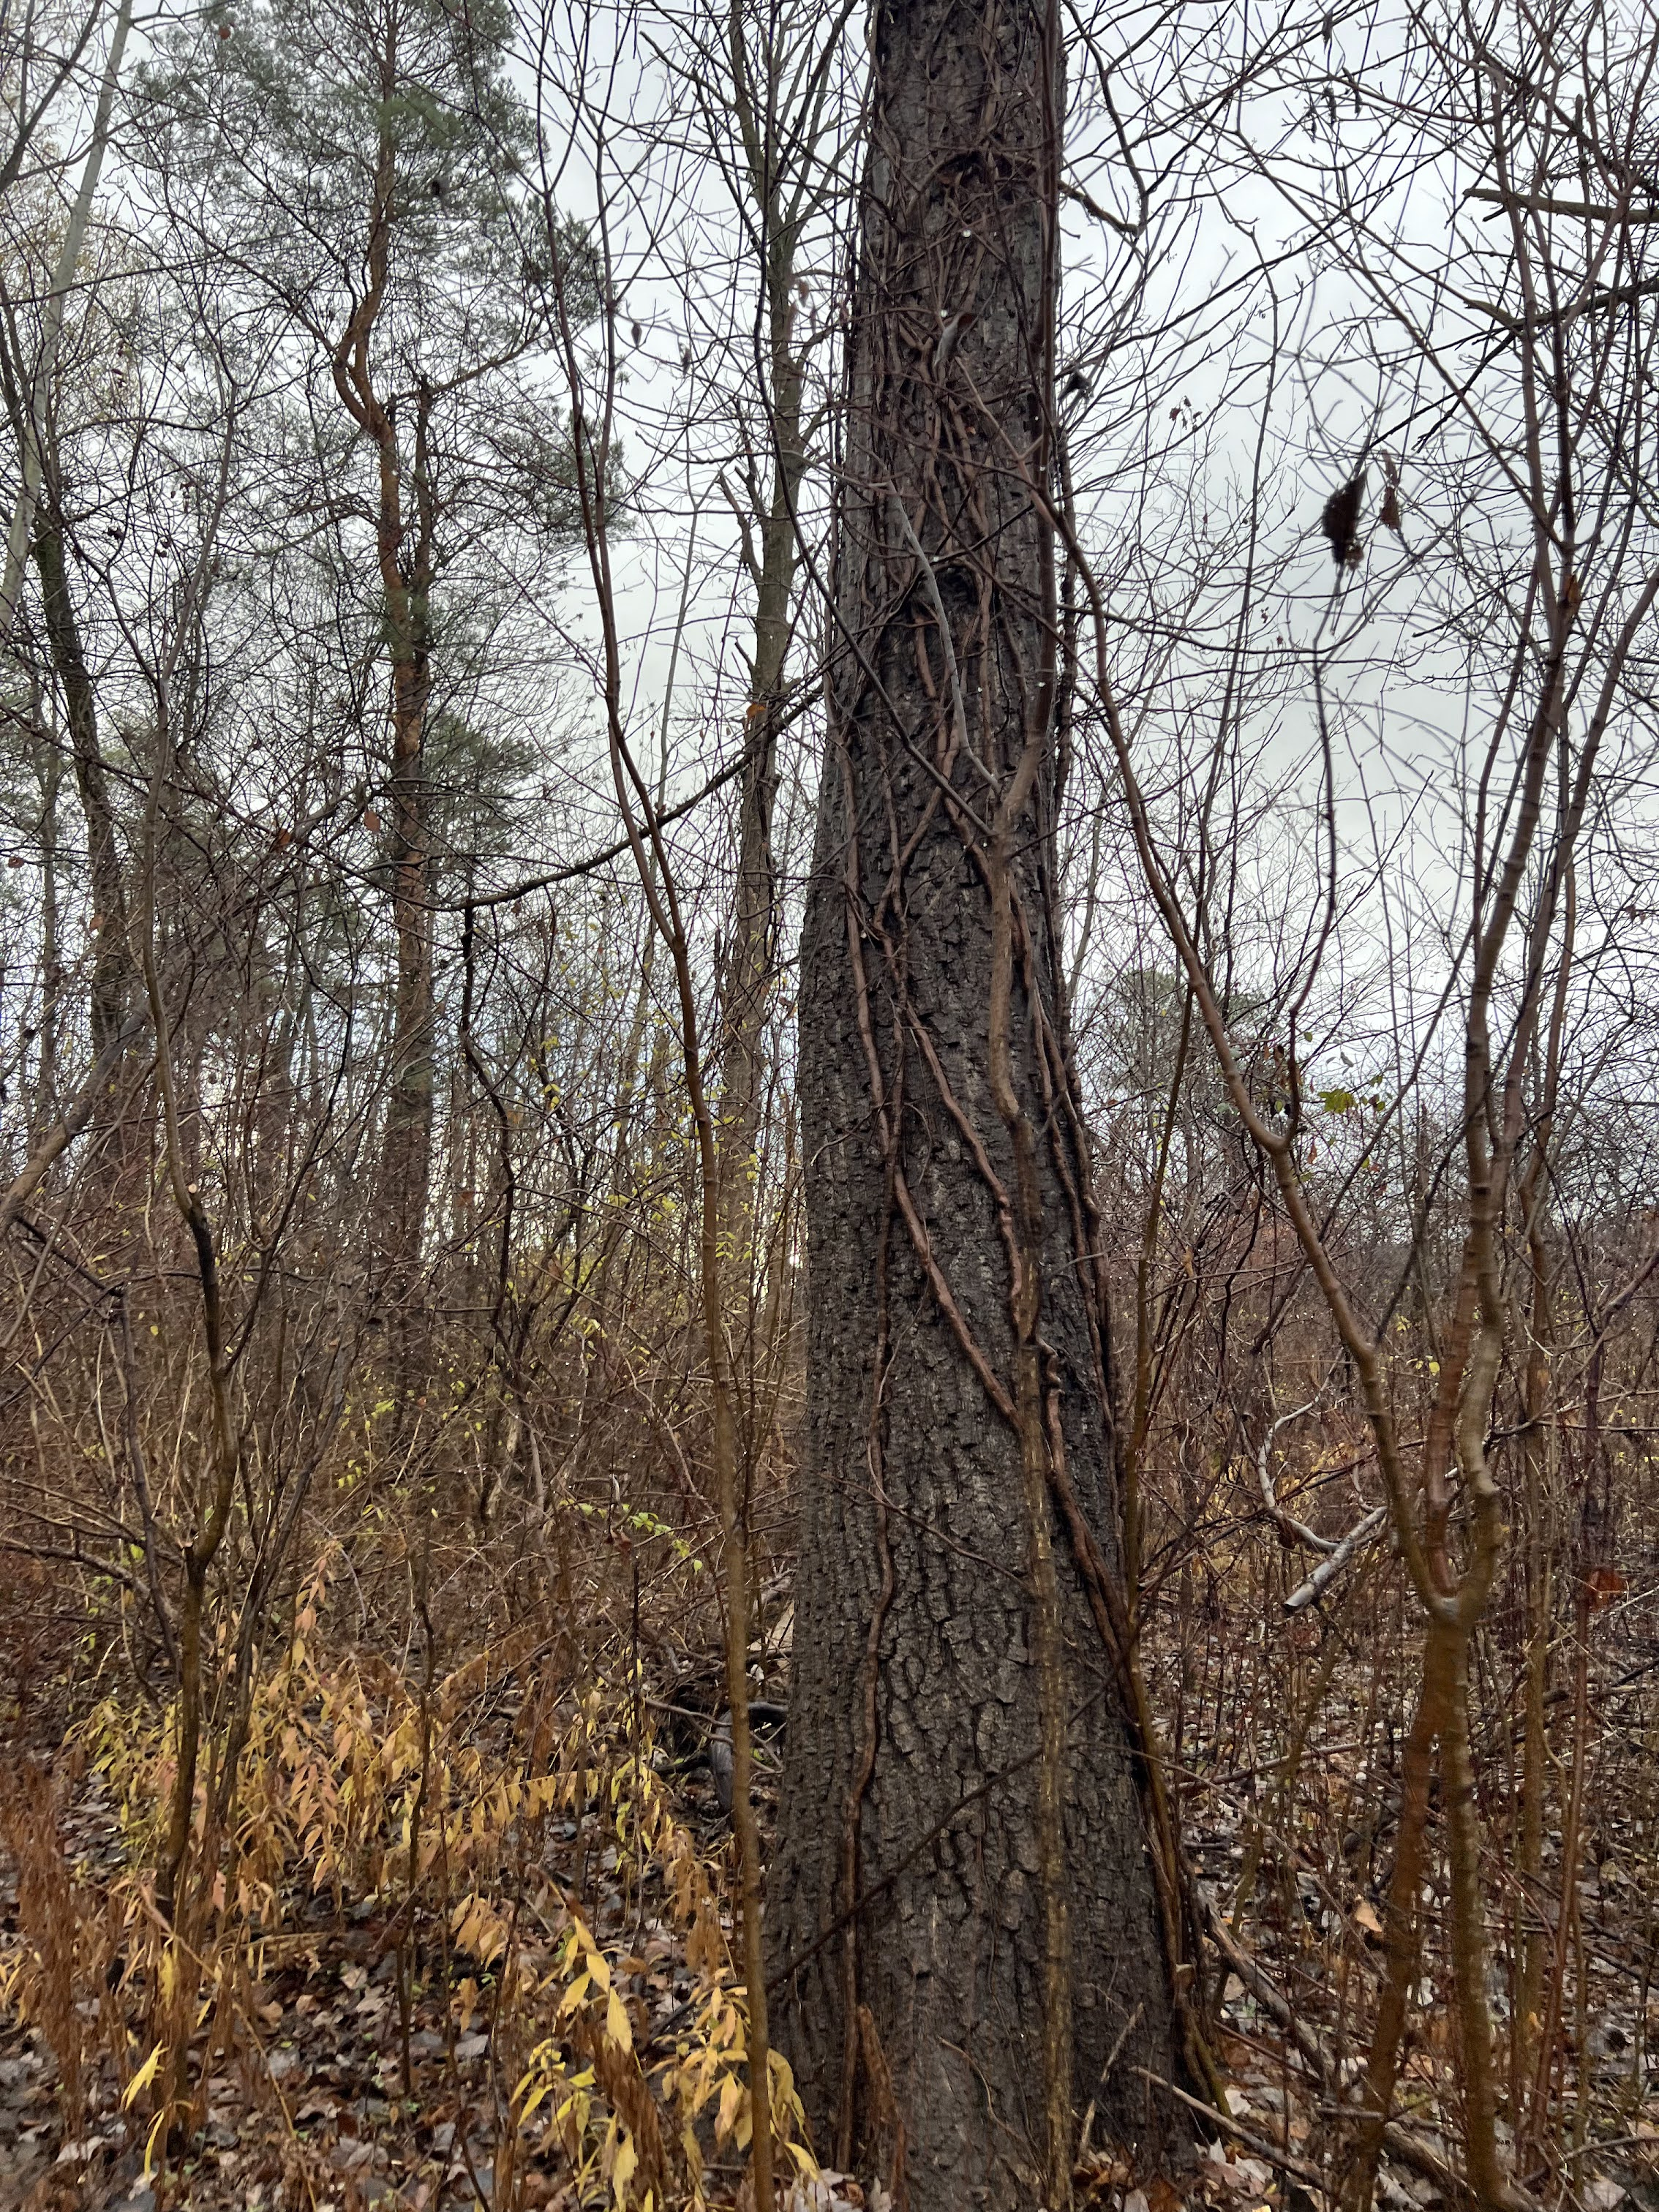
\includegraphics[scale=.1]{Research/HANA/NOV2024/IMG_9856.JPG}
\caption{HANA Tree Study}
\label{fig:HANA}
\end{figure}


\begin{figure}[h!]
\centering
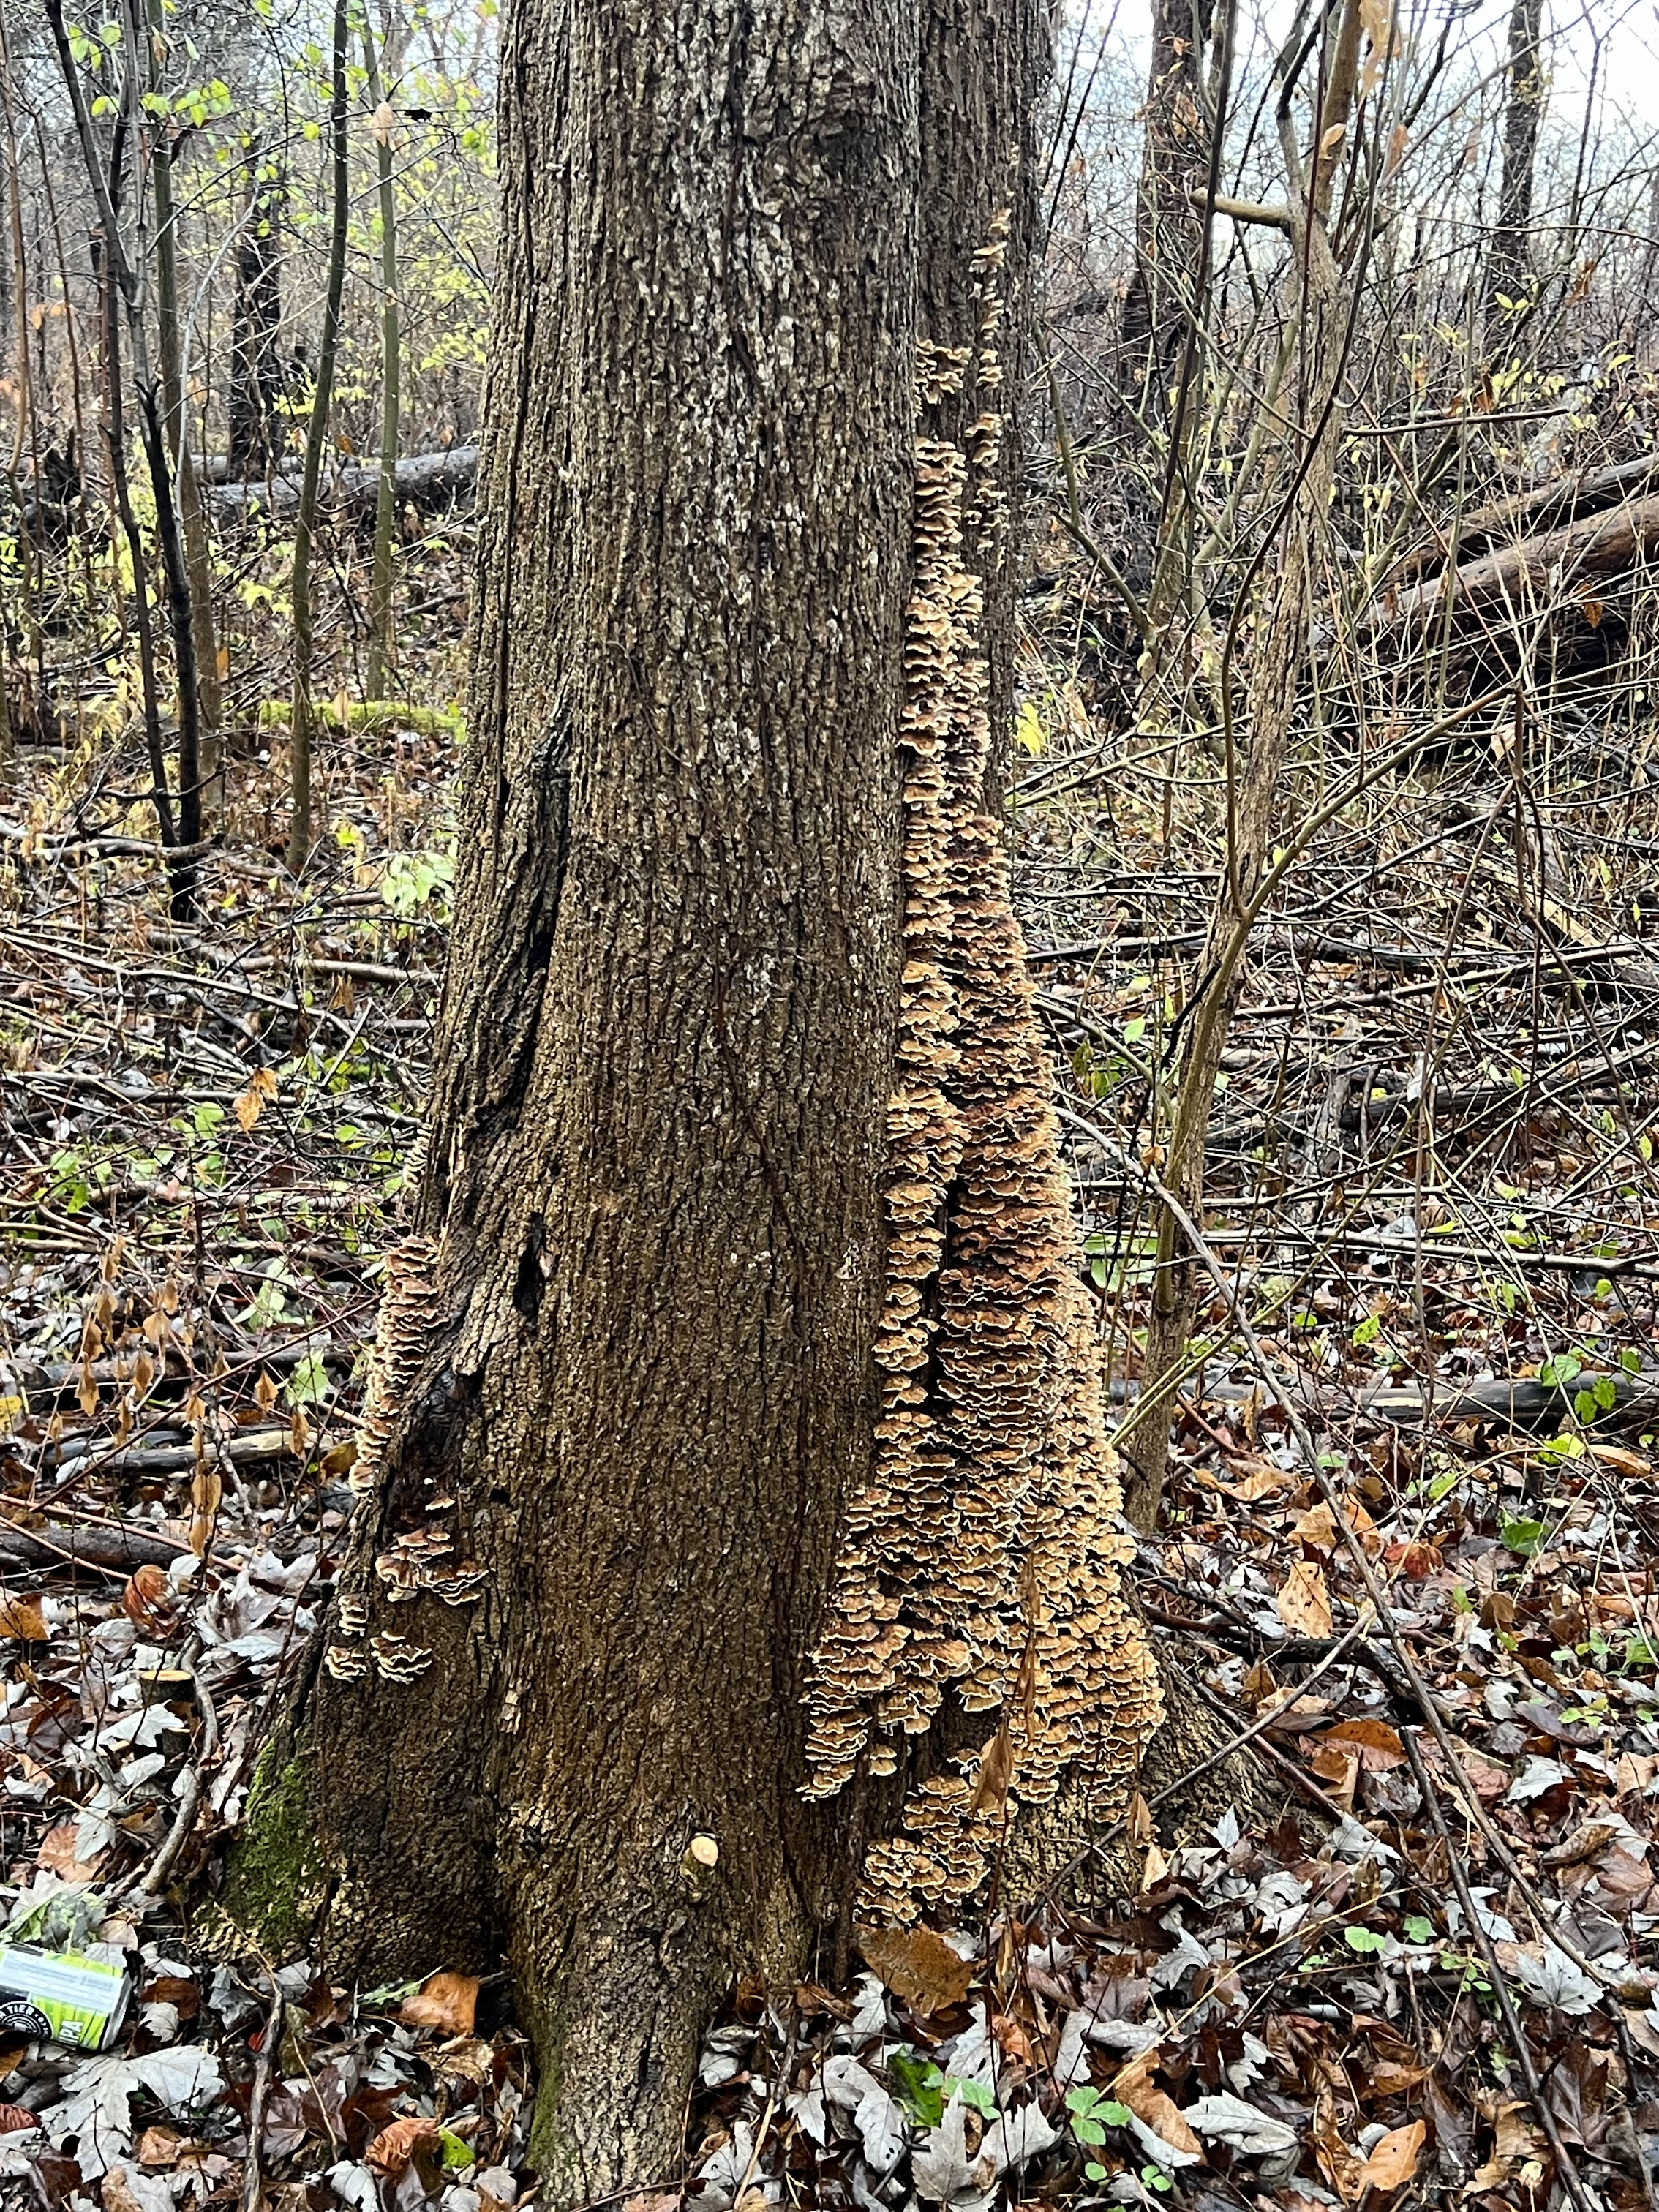
\includegraphics[scale=.1]{Research/HANA/NOV2024/IMG_9859.JPG}
\caption{HANA Tree Study}
\label{fig:HANA}
\end{figure}


\begin{figure}[h!]
\centering
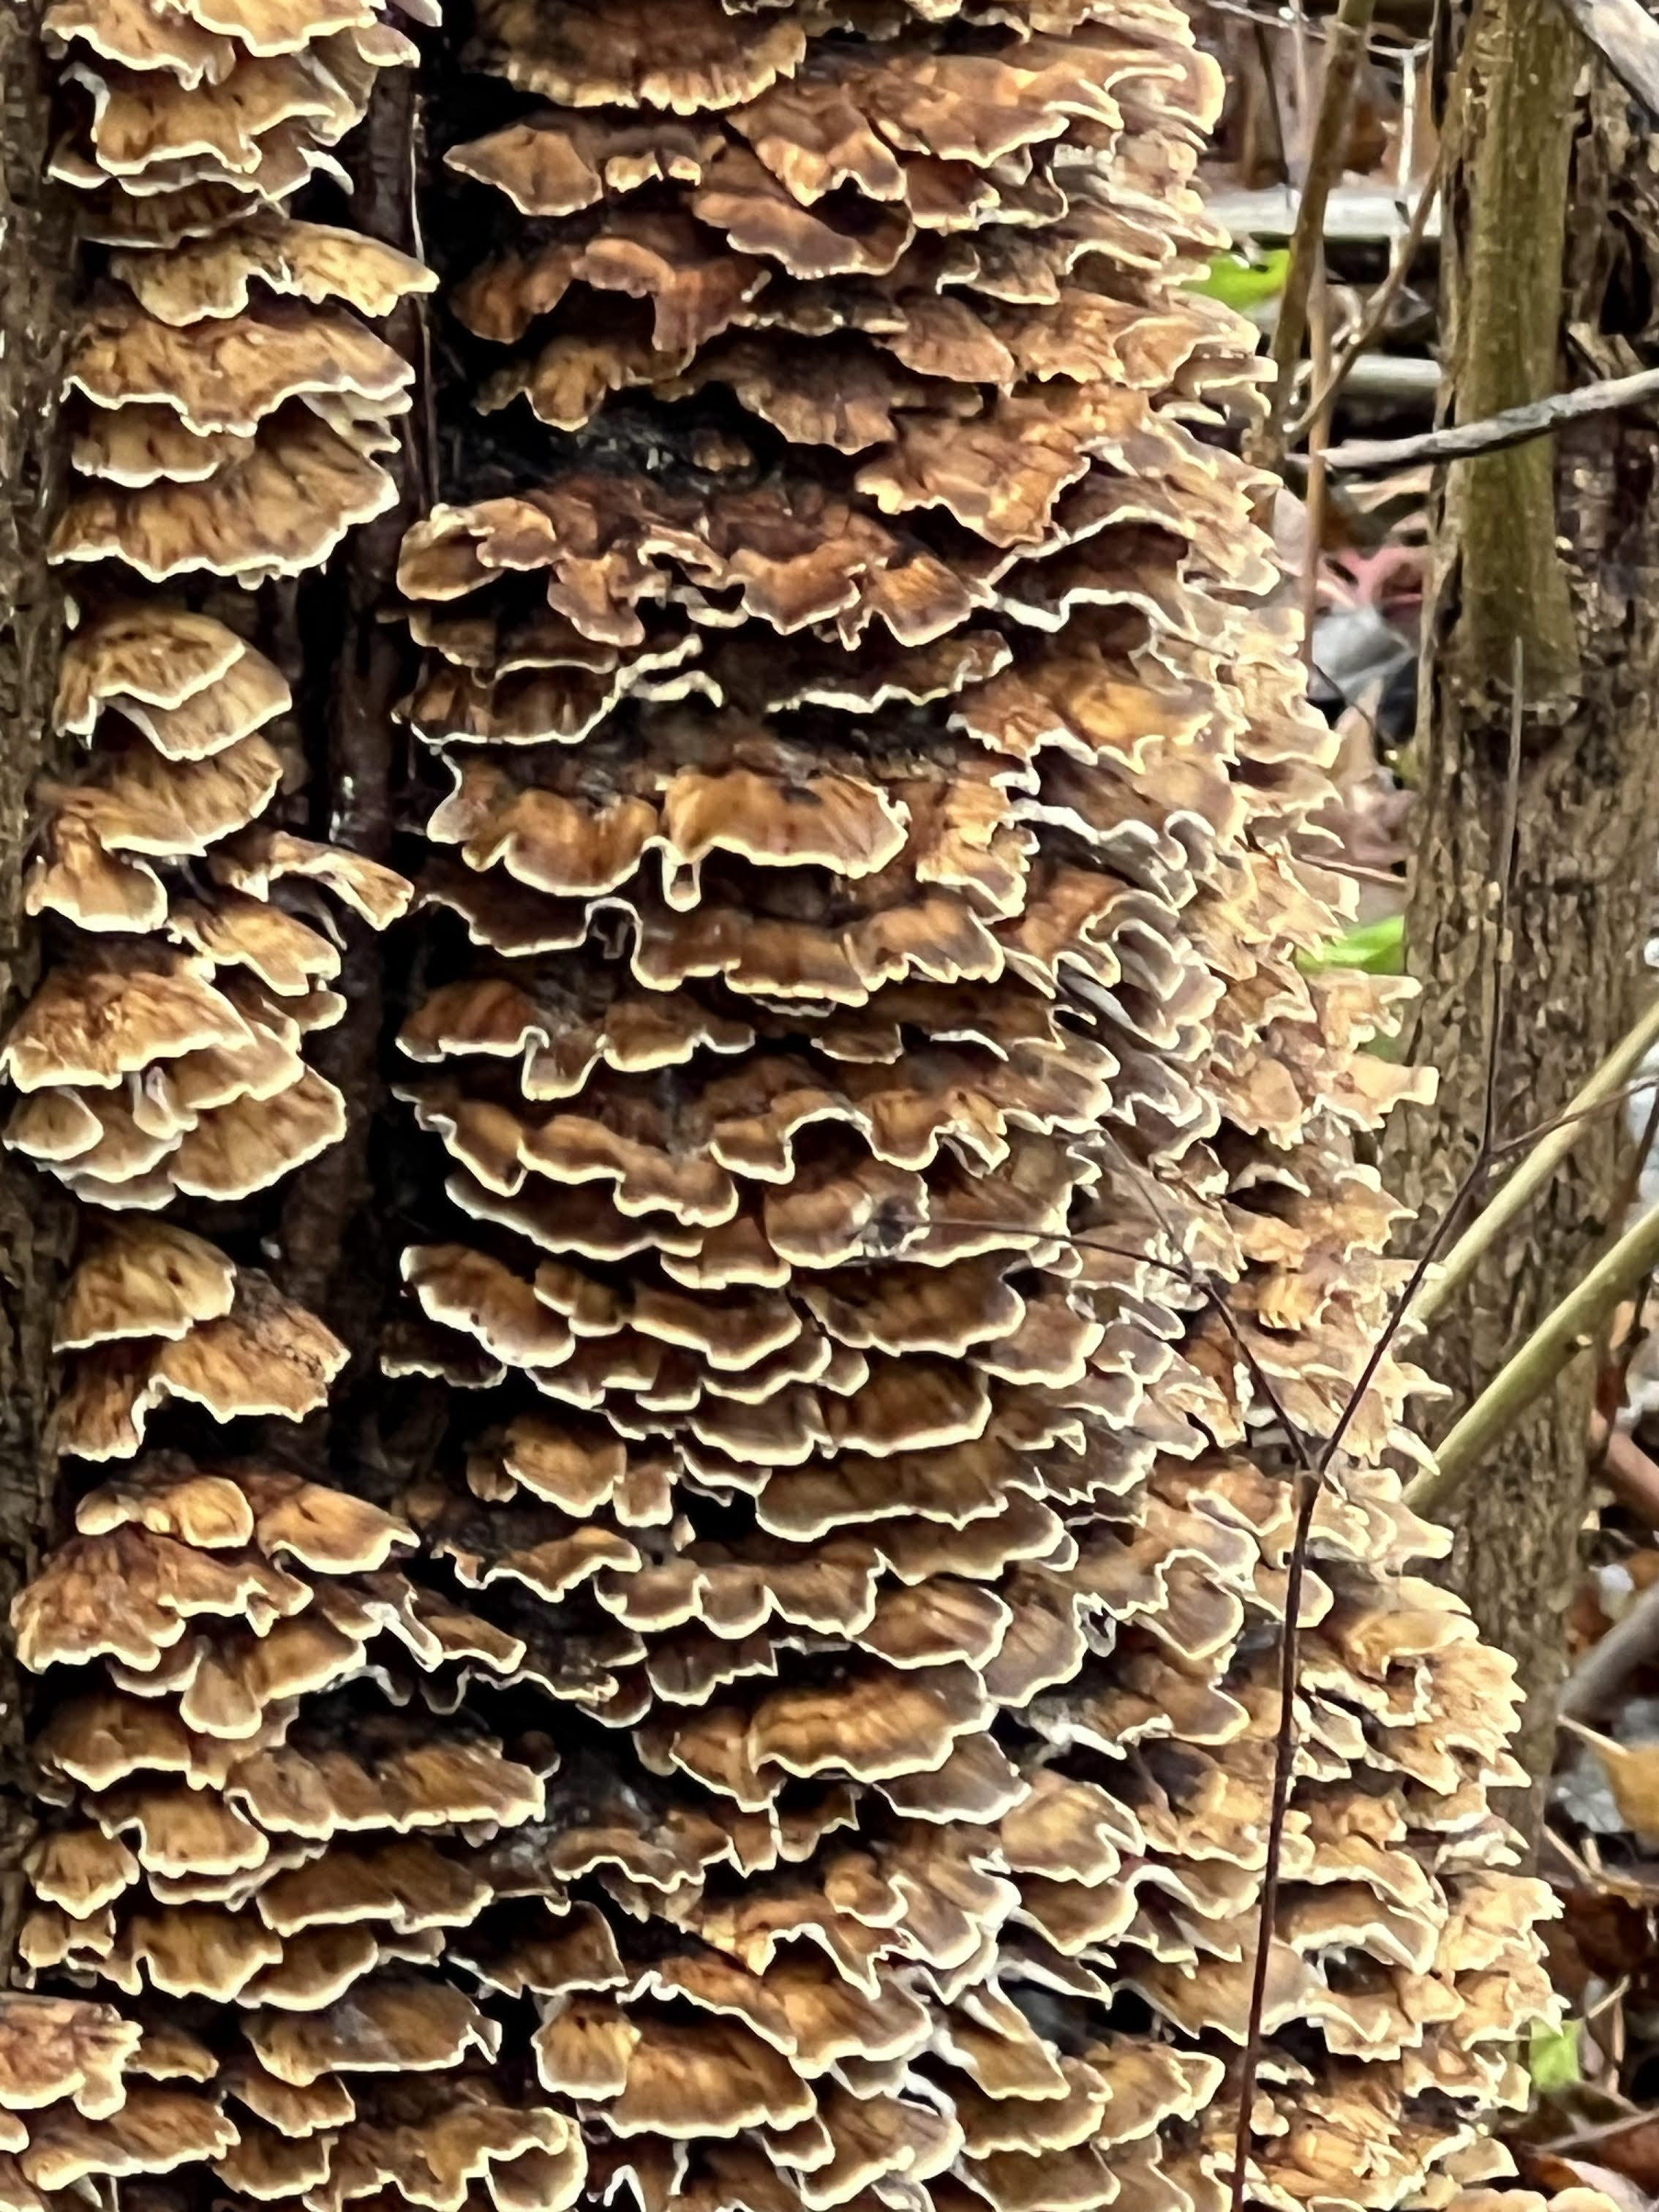
\includegraphics[scale=.1]{Research/HANA/NOV2024/IMG_9860.JPG}
\caption{HANA Tree Study}
\label{fig:HANA}
\end{figure}


\clearpage
\section{Bibliography}
\begin{thebibliography}{}

\bibitem{Calculus}
Stewart, James. Stewart Calculus. Cengage Learning Emea, 2014.

\bibitem{Fourier}
Easton, Roger Jr. Fourier Methods in Imaging. John Wiley and Sons, Incorporated, 2010.


\end{thebibliography}

\end{document}



